\section{Results}
\label{sec:results}


\subsection{Local Fractal Dimension of Datasets}
\label{sec:results:lfd-of-datasets}

Since the time complexity of CAKES algorithms scales with the LFD of the dataset, we examine the LFD of each dataset we used for benchmarks.
Figure~\ref{fig:results:lfd-plots} illustrates the trends in LFD for Fashion-Mnist, Glove-25, Sift, Random, Silva 18S, and RadioML.
The horizontal axis denotes depth in the cluster tree, and the vertical axis denotes the LFD of clusters at that depth.
We plot lines for the 5$^{th}$, 25$^{th}$, 50th, 75$^{th}$ and 95$^{th}$ percentiles of LFD, as well as the minimum and maximum LFD at each depth.
In order to have the plots best reflect the distribution of LFDs across the entire \textit{dataset}, we count each cluster as many times as its cardinality.
In other words, if, for some dataset, the 95$^{th}$ percentile of LFD at depth 40 is 3, this means that 95\% of the points in clusters at depth 40 belong to a cluster whose LFD is at most 3.
Figure~\ref{fig:results:fashion-mnist-lfd} shows the LFD by depth for Fashion-Mnist.
We observe that until about depth 5, LFD is low, as the 95$^{th}$ percentile (orange plotted line) is less than 4, and the median (red line) is just above 2.
For depths 15 through 25, we observe that LFD increases, with the 95$^{th}$ percentile (orange plotted line) slightly less than 6, and the median near 3.
Finally, for depths 25 through the maximum depth, we observe that the LFD decreases again, as the 95$^{th}$ percentile is between 3 and 4, and the median is less than 2.

Relative to Fashion-Mnist, Glove-25 has low LFD, as shown in Figure~\ref{fig:results:glove-25-lfd}.
Percentile lines for Glove-25 are flatter and lower, indicating that the LFD is lower across the entire dataset, and that the LFD does not vary as much by depth.
The 95$^{th}$ percentile of LFD is less than 3 for all depths, and the median is less than 2 for all depths.
Before depth 25, the 95$^{th}$ percentile hovers near 2, and from depth 20 onward, it hovers near 3.5 before dipping sharply at the maximum depths.
The median hovers near 1.5 for all depths.

Figure~\ref{fig:results:sift-lfd} shows the LFD by depth for Sift.
Until about depth 5, the 95$^{th}$ percentile is between 2 and 6.
From about depth 5 through about depth 20, the 95$^{th}$ percentile is greater than 6, even exceeding 8 near depth 10.
From about depth 20 onward, the 95$^{th}$ percentile is less than 6, and from about depth 30 onward, it is between 3 and 4.
The median reaches its peak of about 5 at around depth 15, but hovers near 2 after about depth 30.

In contrast with Figure~\ref{fig:results:sift-lfd}, Figure~\ref{fig:results:random-lfd} shows the LFD by depth for a random dataset with the same cardinality and dimensionality as those of Sift.
We observe that the LFD starts as high as 20 (for all data) at depth 0.
As shown by the needlepoint shape of the plot, the LFD for all clusters has a very narrow spread from depth 0 through depth 5.
After depth 5, we begin to see a wider spread between the maximum and minimum LFD at each depth.
All percentile lines seem to decrease linearly with depth.
The LFD of approximately 20 at depth 0 (i.e.,\,the root cluster) is what we expect for this random dataset.
To elaborate, the distribution of points in such a dataset should reflect the curse of dimensionality, i.e.,\,the fact that in high dimensional spaces, the minimum and maximum pairwise distances between any two points are approximately equal.
As a result, the root cluster's radius $r$, which reflects the maximum distance between the center $c$ and any other point, should not differ significantly from the distance between the center and its closest point.
A consequence of this is that, with high probability, for every point in the root cluster, its distance from $c$ is greater than $\tfrac{r}{2}$;
in other words, $B_X(c, \tfrac{r}{2})$ contains only $c$ while $B_X(c, r)$ contains the entire dataset.
Given our definition of LFD in Equation~\ref{eq:methods:lfd-original}, this means that the LFD of the root cluster is approximately $\log_2(\frac{|X|}{1}) = \log_2(1,000,000) \approx 20$, which is what we observe in Figure~\ref{fig:results:random-lfd}.

Silva, as shown in Figure~\ref{fig:results:silva-lfd}, exhibits consistently low LFD.
The 95$^{th}$ percentile is less than about 3 for all depths, hovering near 1 for depths 40 through 128.
The median reaches its peak at 2 for about depth 10 and remains close to 0 for depths 40 through 128.

Relative to the other datasets, RadioML, as displayed in Figure~\ref{fig:results:radioml-lfd}, exhibits high LFD.
Notably, however, for the first approximately 15 depths, the 95$^{th}$ percentile and median LFD are very close to 0.
Both percentiles increase sharply after depth 20, nearly reaching 16.
LFD remains high even as depth increases, with the 95$^{th}$ percentile fluctuating between about 6 and 15 for depths about 20-40.
It then spikes up again to about 10 at around depth 45 before decreasing linearly to 1 at depth 60.
The median LFD follows a similar pattern of peaks and troughs, fluctuating between about 3 and 15 for depths 20-40, spiking at about depth 50 to 5, and then decreasing approximately linearly to 1 at depth 60. The inconsistency of LFD in the RadioML dataset suggests that it obeys the manifold hypothesis at some scales, but that it is not ``scale free,'' as the LFD varies significantly by depth; this could be due to dense sampling or---as this is still a synthetic dataset---nonuniform generation of data. Silva, in contrast, appears to obey the manifold hypothesis at all scales.

\begin{figure}
    \begin{subfigure}[b]{0.47\textwidth}
        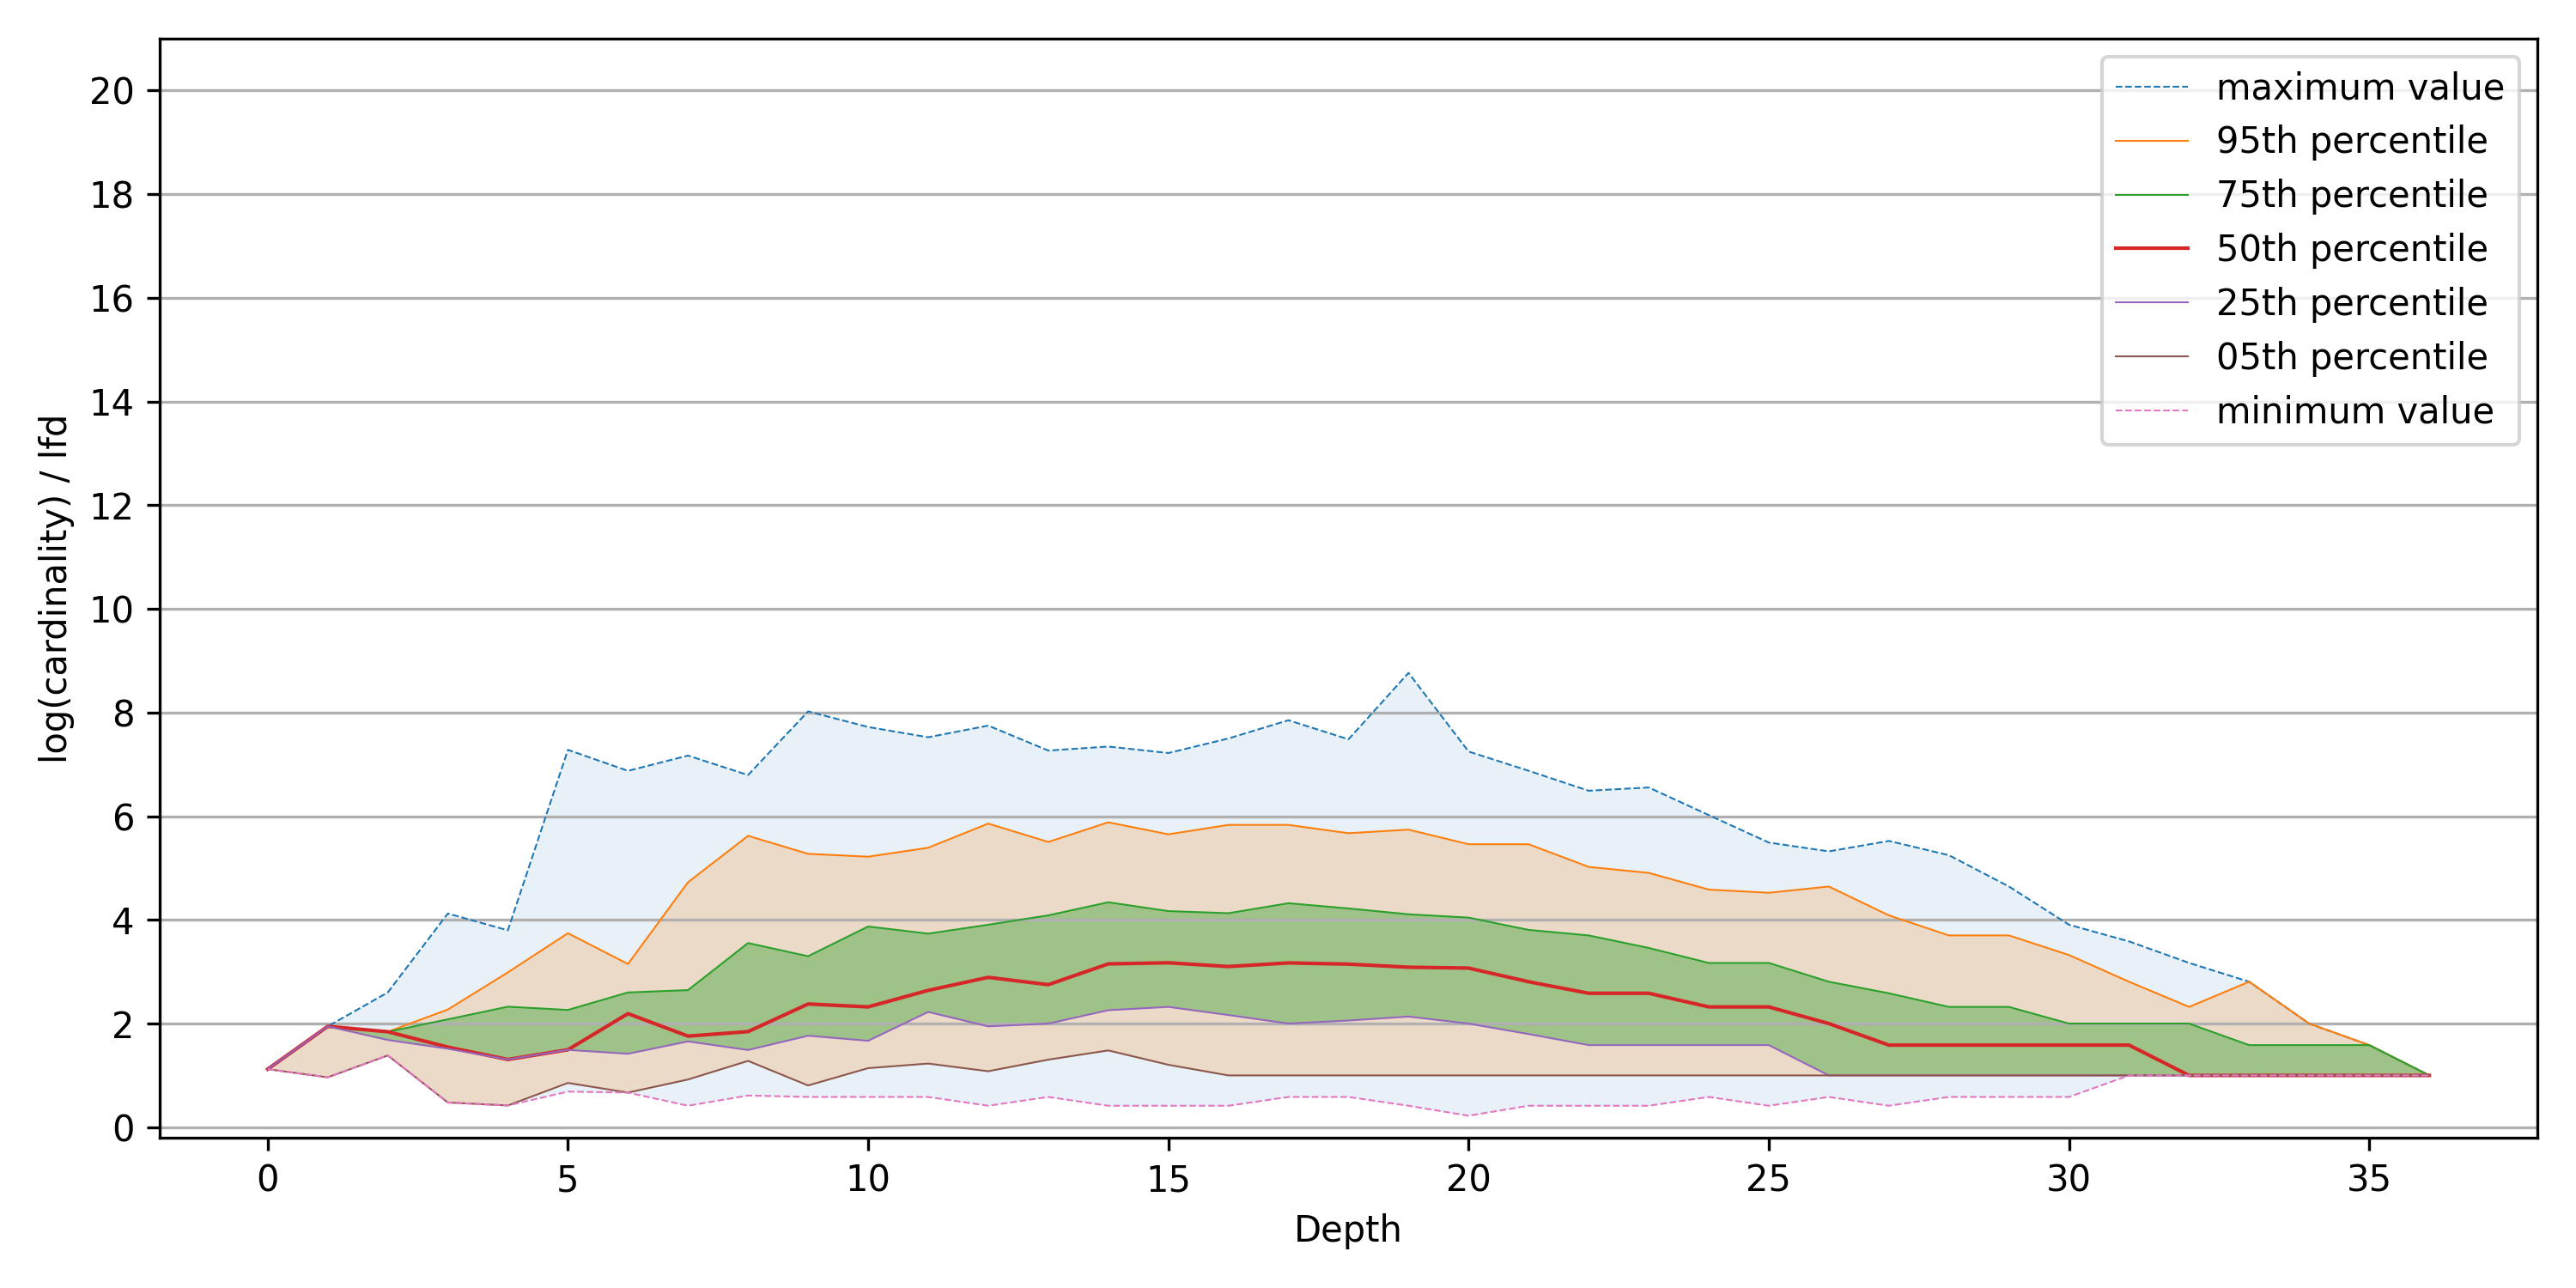
\includegraphics[width=0.95\textwidth]{images/lfd/fashion-mnist-60000.png}\\
        \subcaption{Fashion-mnist}
        \label{fig:results:fashion-mnist-lfd}
    \end{subfigure}%
    \begin{subfigure}[b]{0.47\textwidth}
        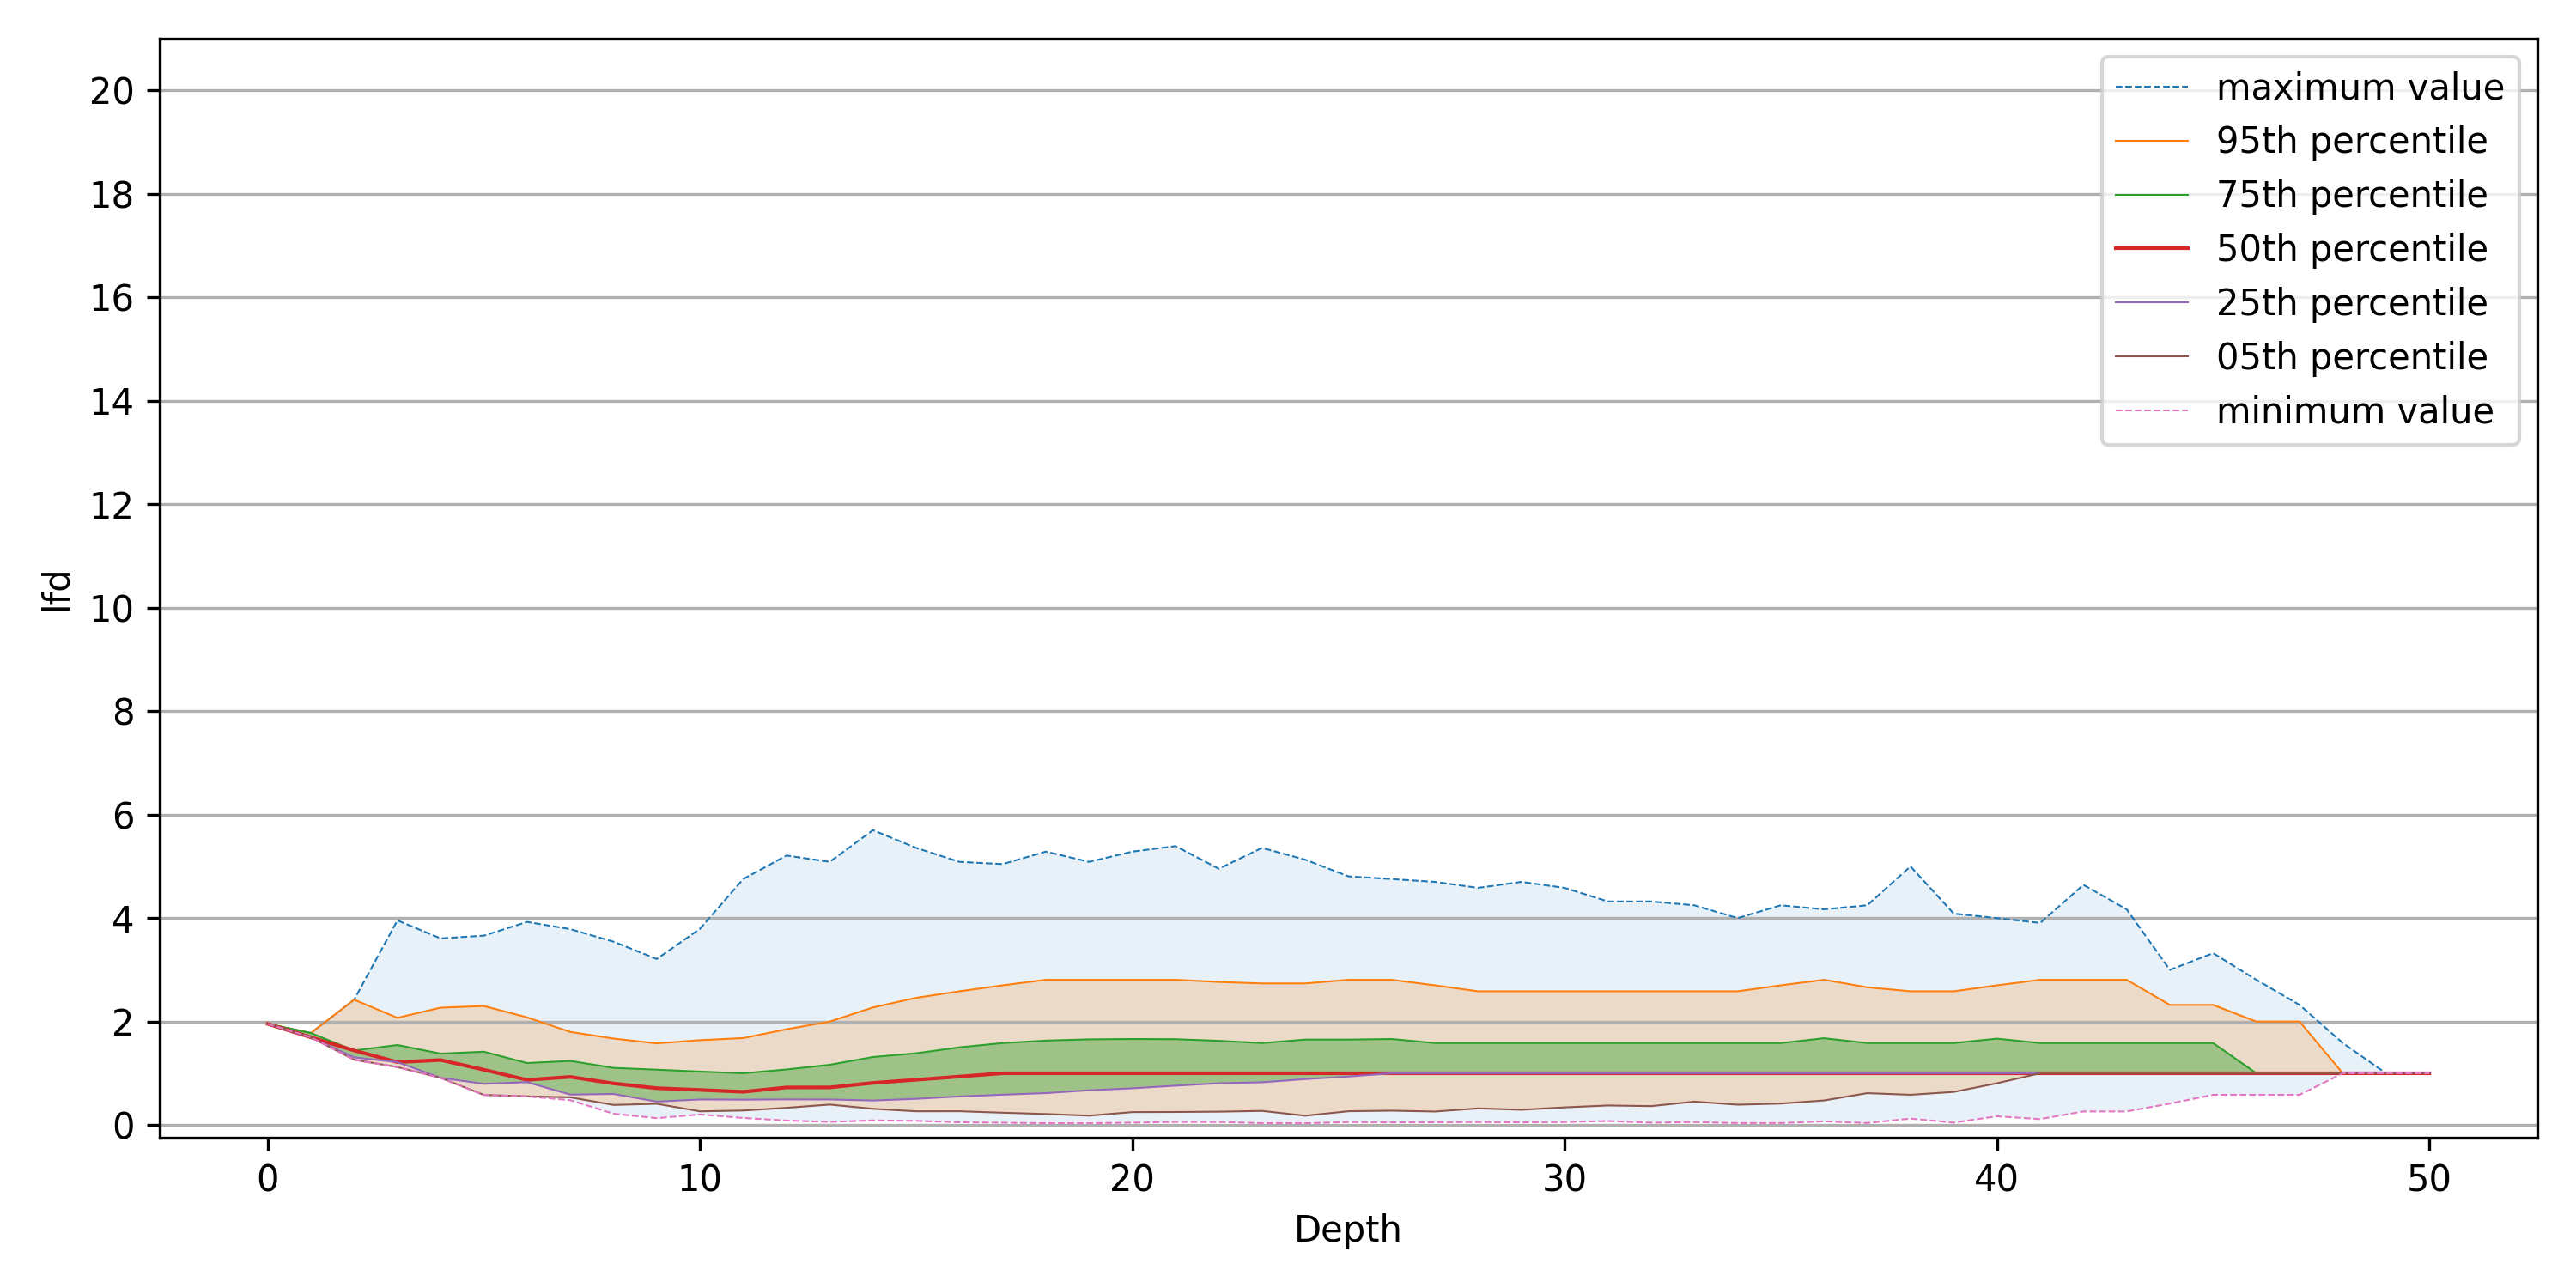
\includegraphics[width=0.95\textwidth]{images/lfd/glove-25-1183514.png}\\
        \subcaption{Glove-25}
        \label{fig:results:glove-25-lfd}
    \end{subfigure}
    \vspace{1em}
    \\
    \begin{subfigure}[b]{0.47\textwidth}
        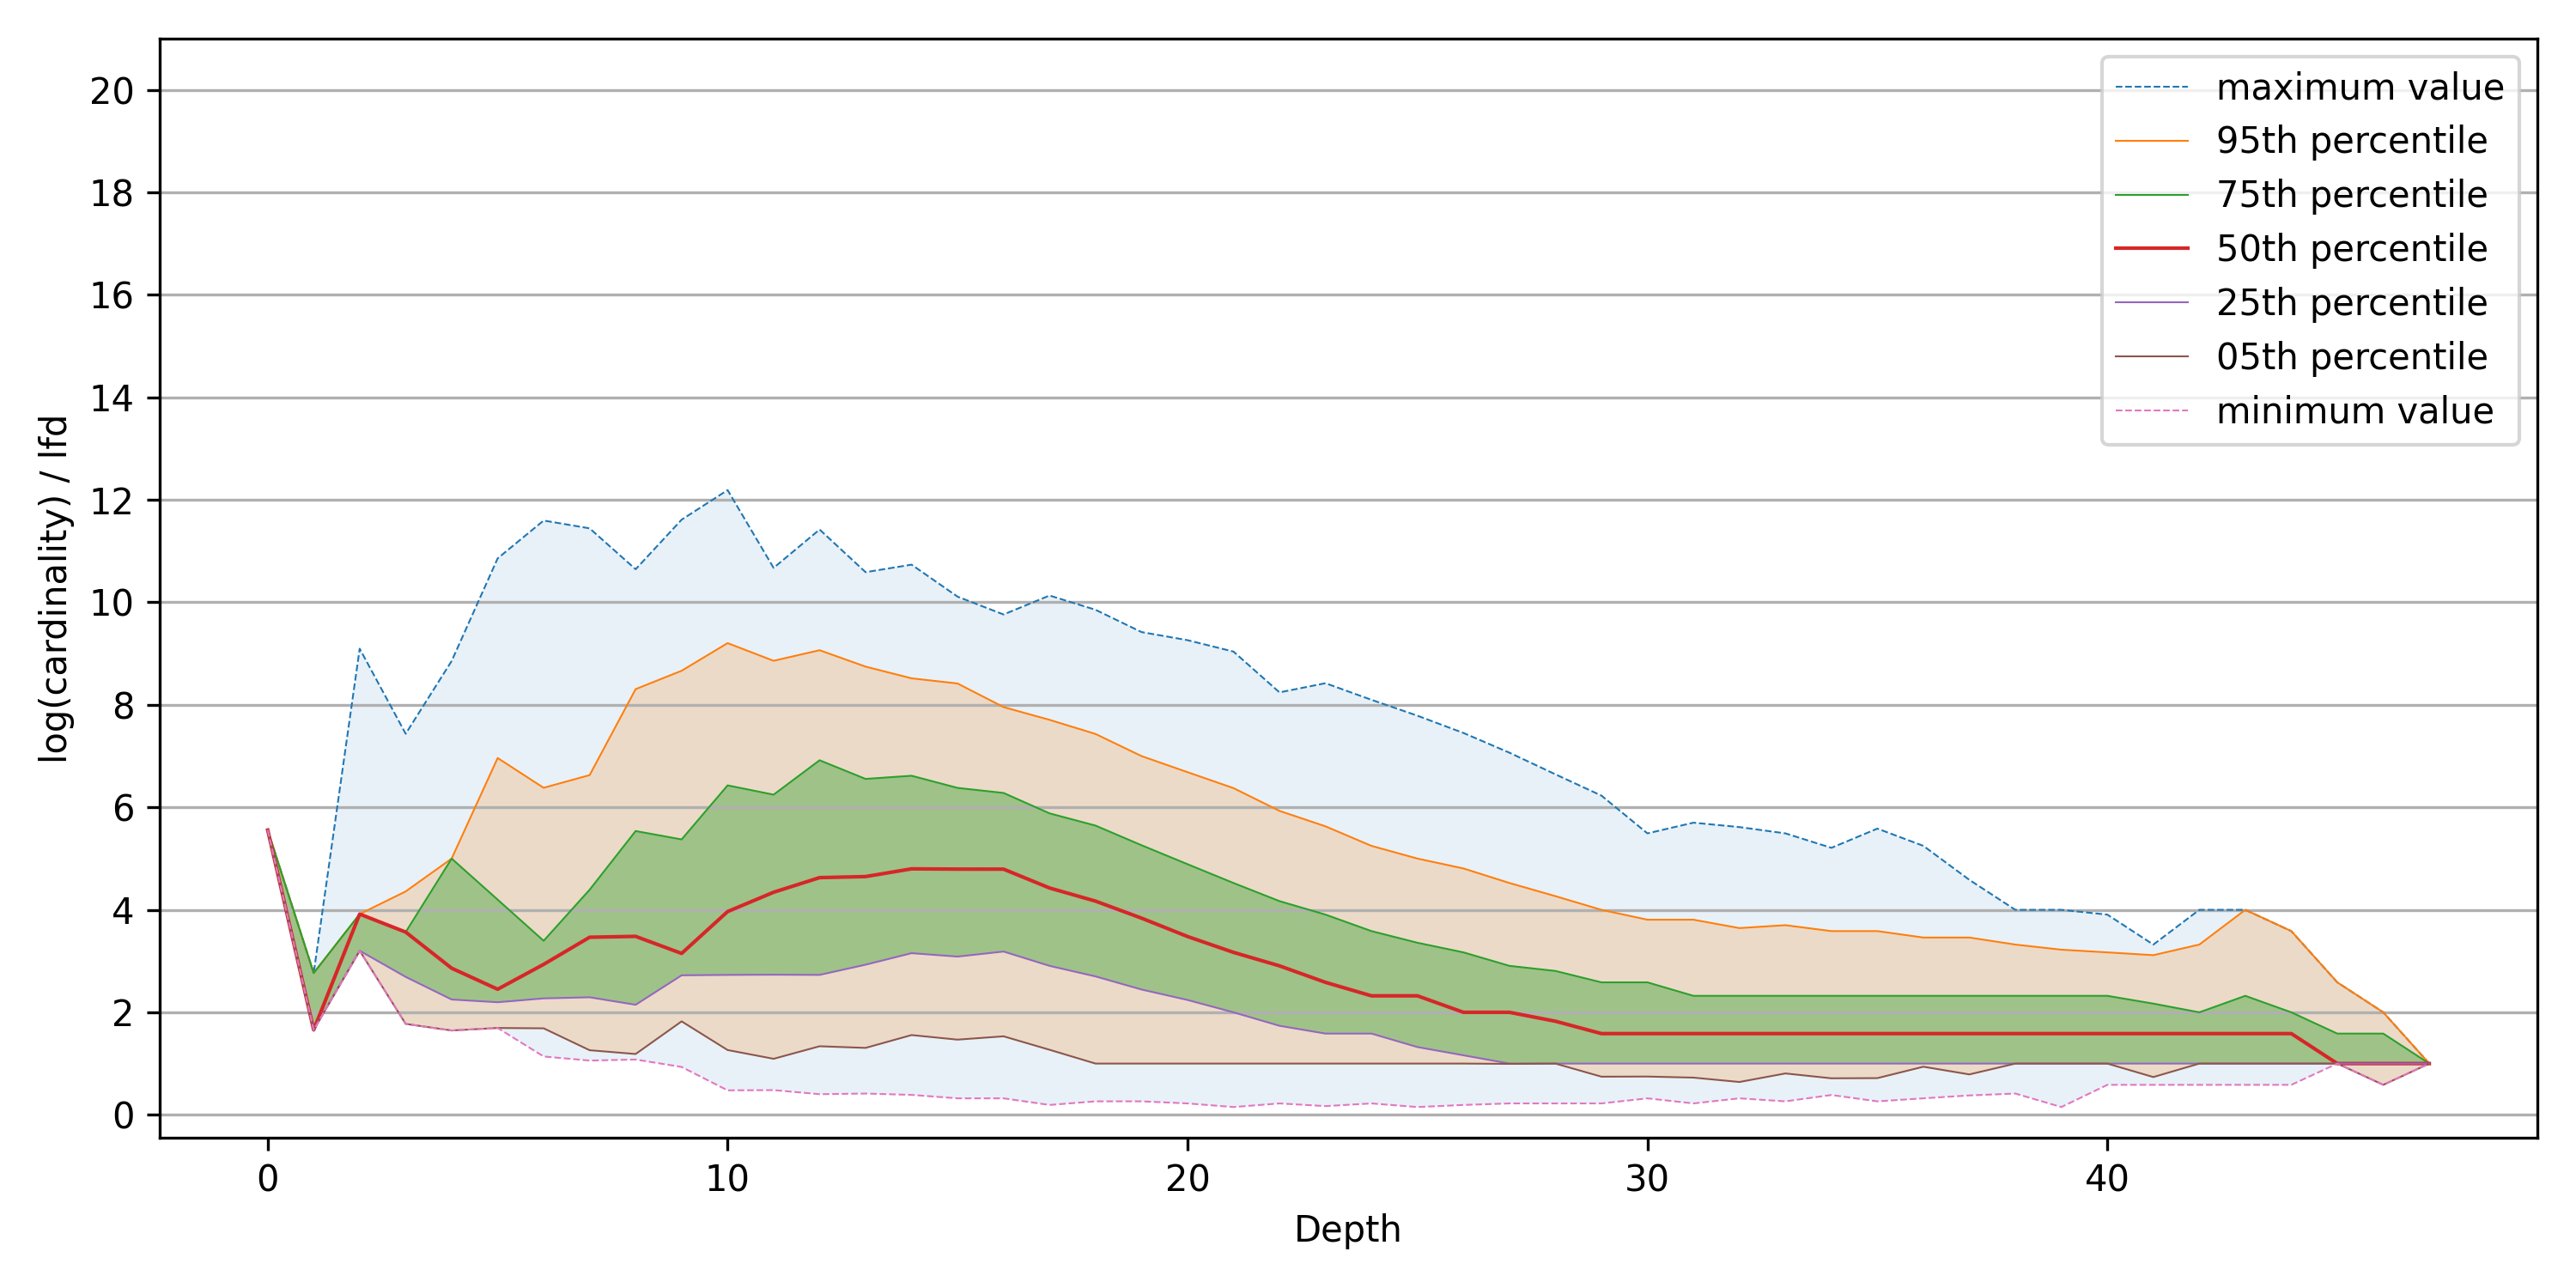
\includegraphics[width=0.95\textwidth]{images/lfd/sift-1000000.png}\\
        \subcaption{Sift}
        \label{fig:results:sift-lfd}
    \end{subfigure}%
    \begin{subfigure}[b]{0.47\textwidth}
        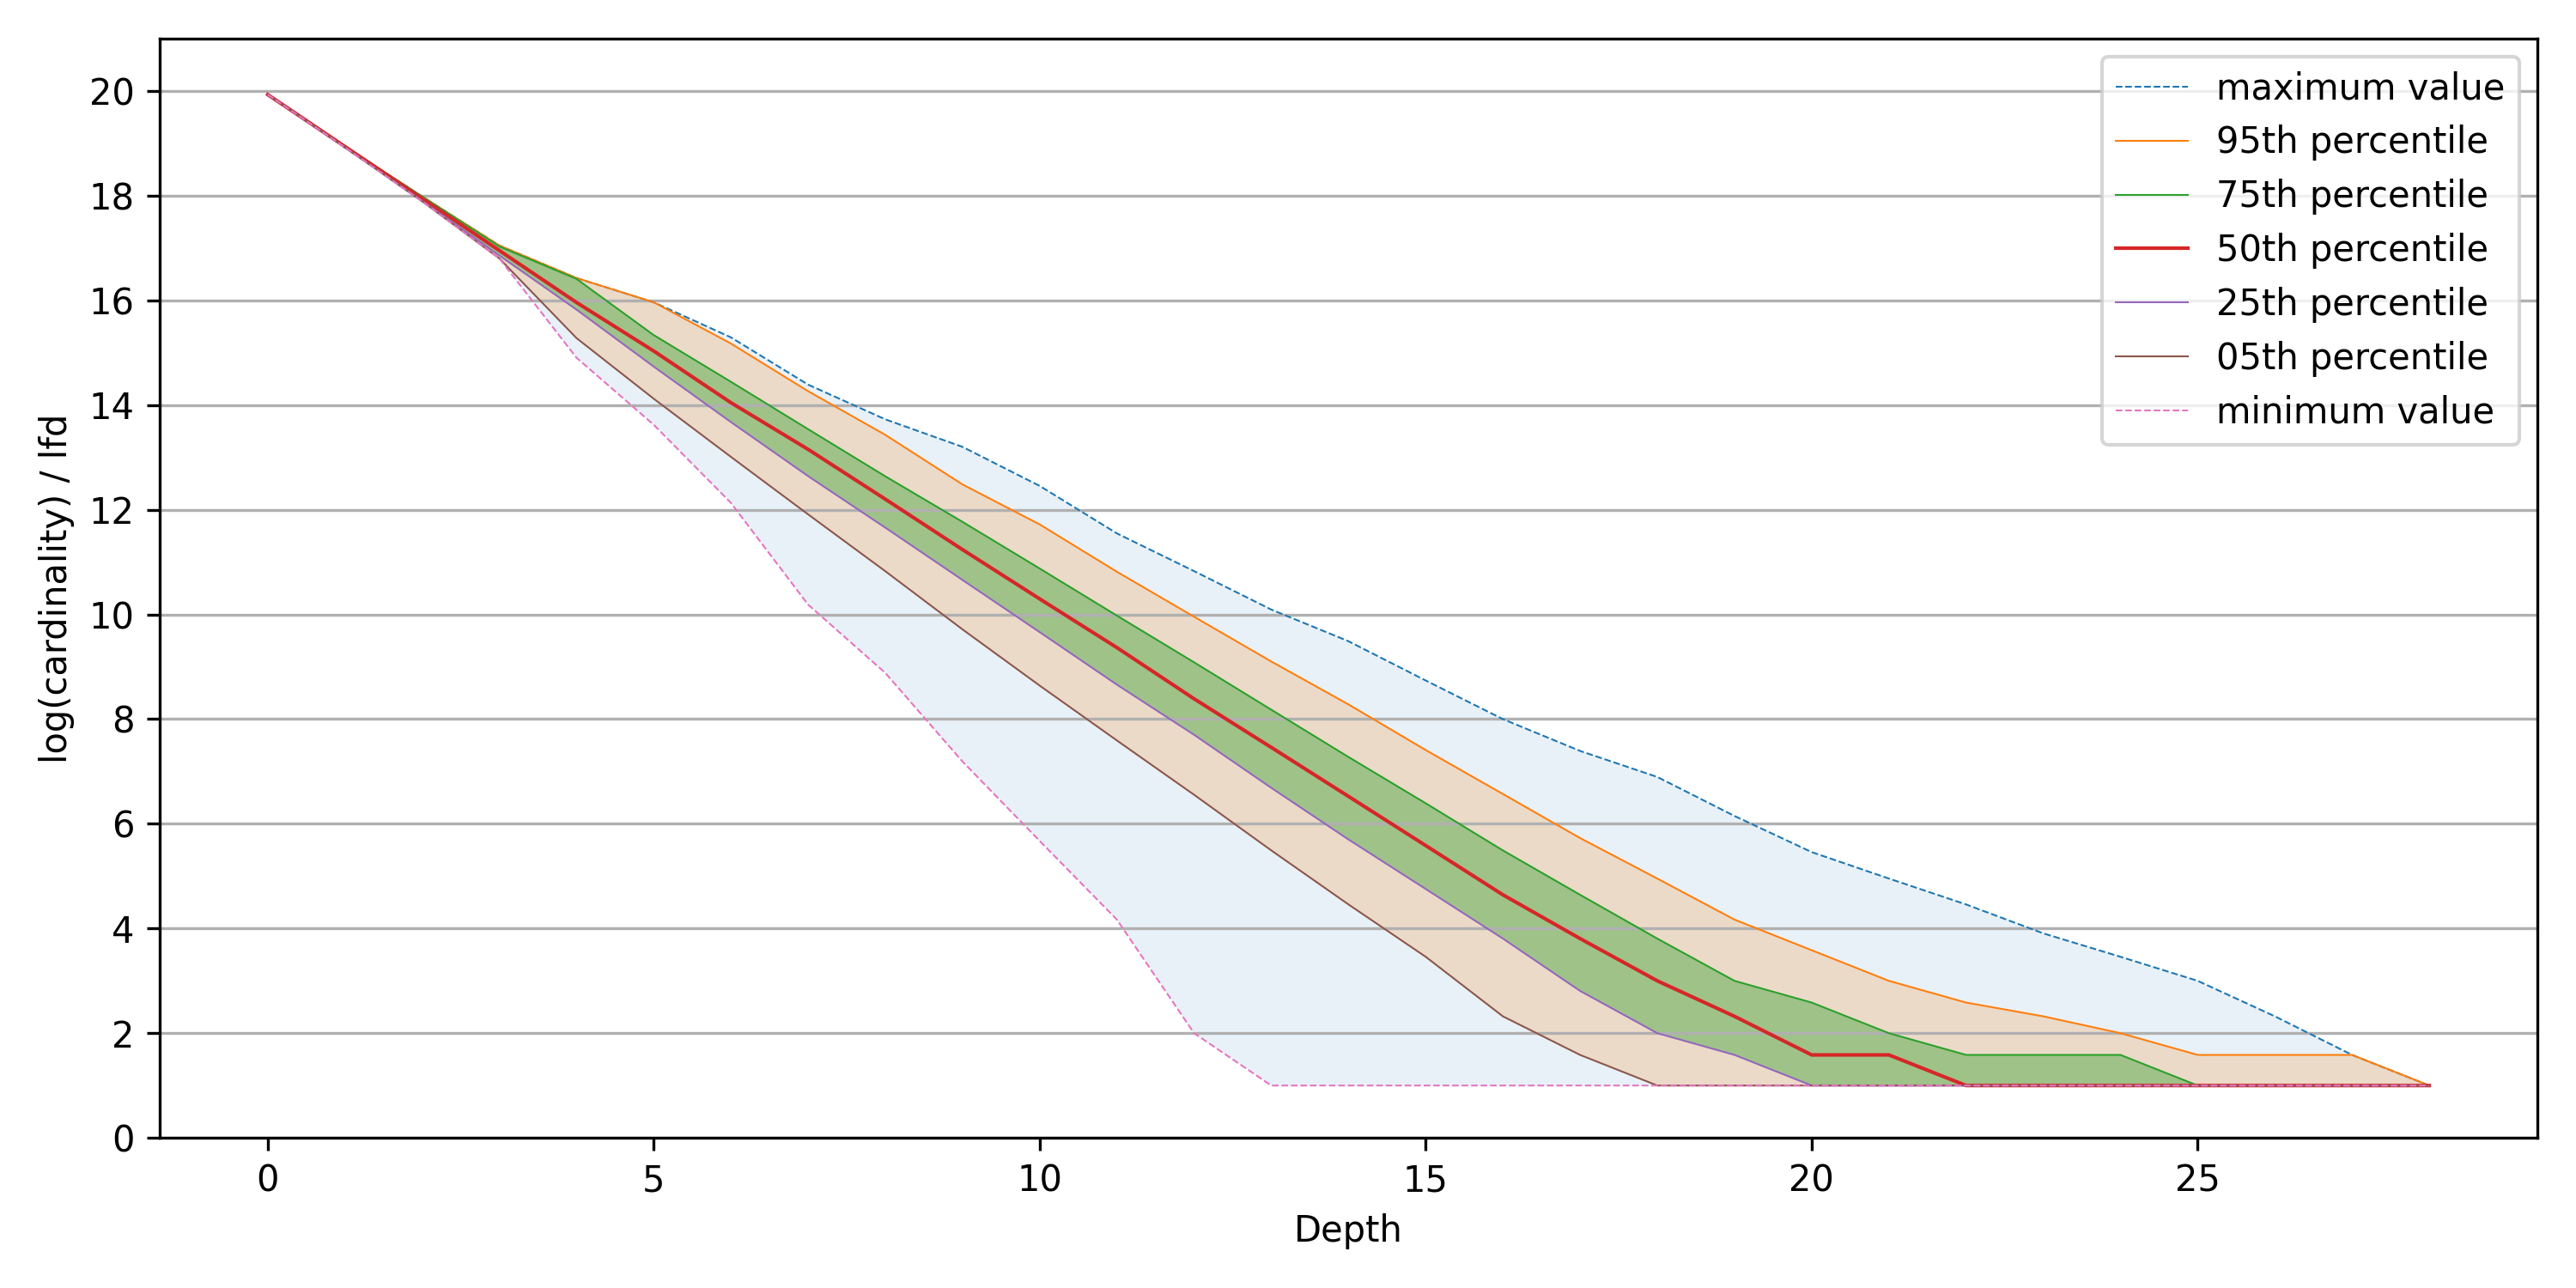
\includegraphics[width=0.95\textwidth]{images/lfd/random-1000000.png}\\
        \subcaption{A random dataset}
        \label{fig:results:random-lfd}
    \end{subfigure}
    \\
    \begin{subfigure}[b]{0.47\textwidth}
        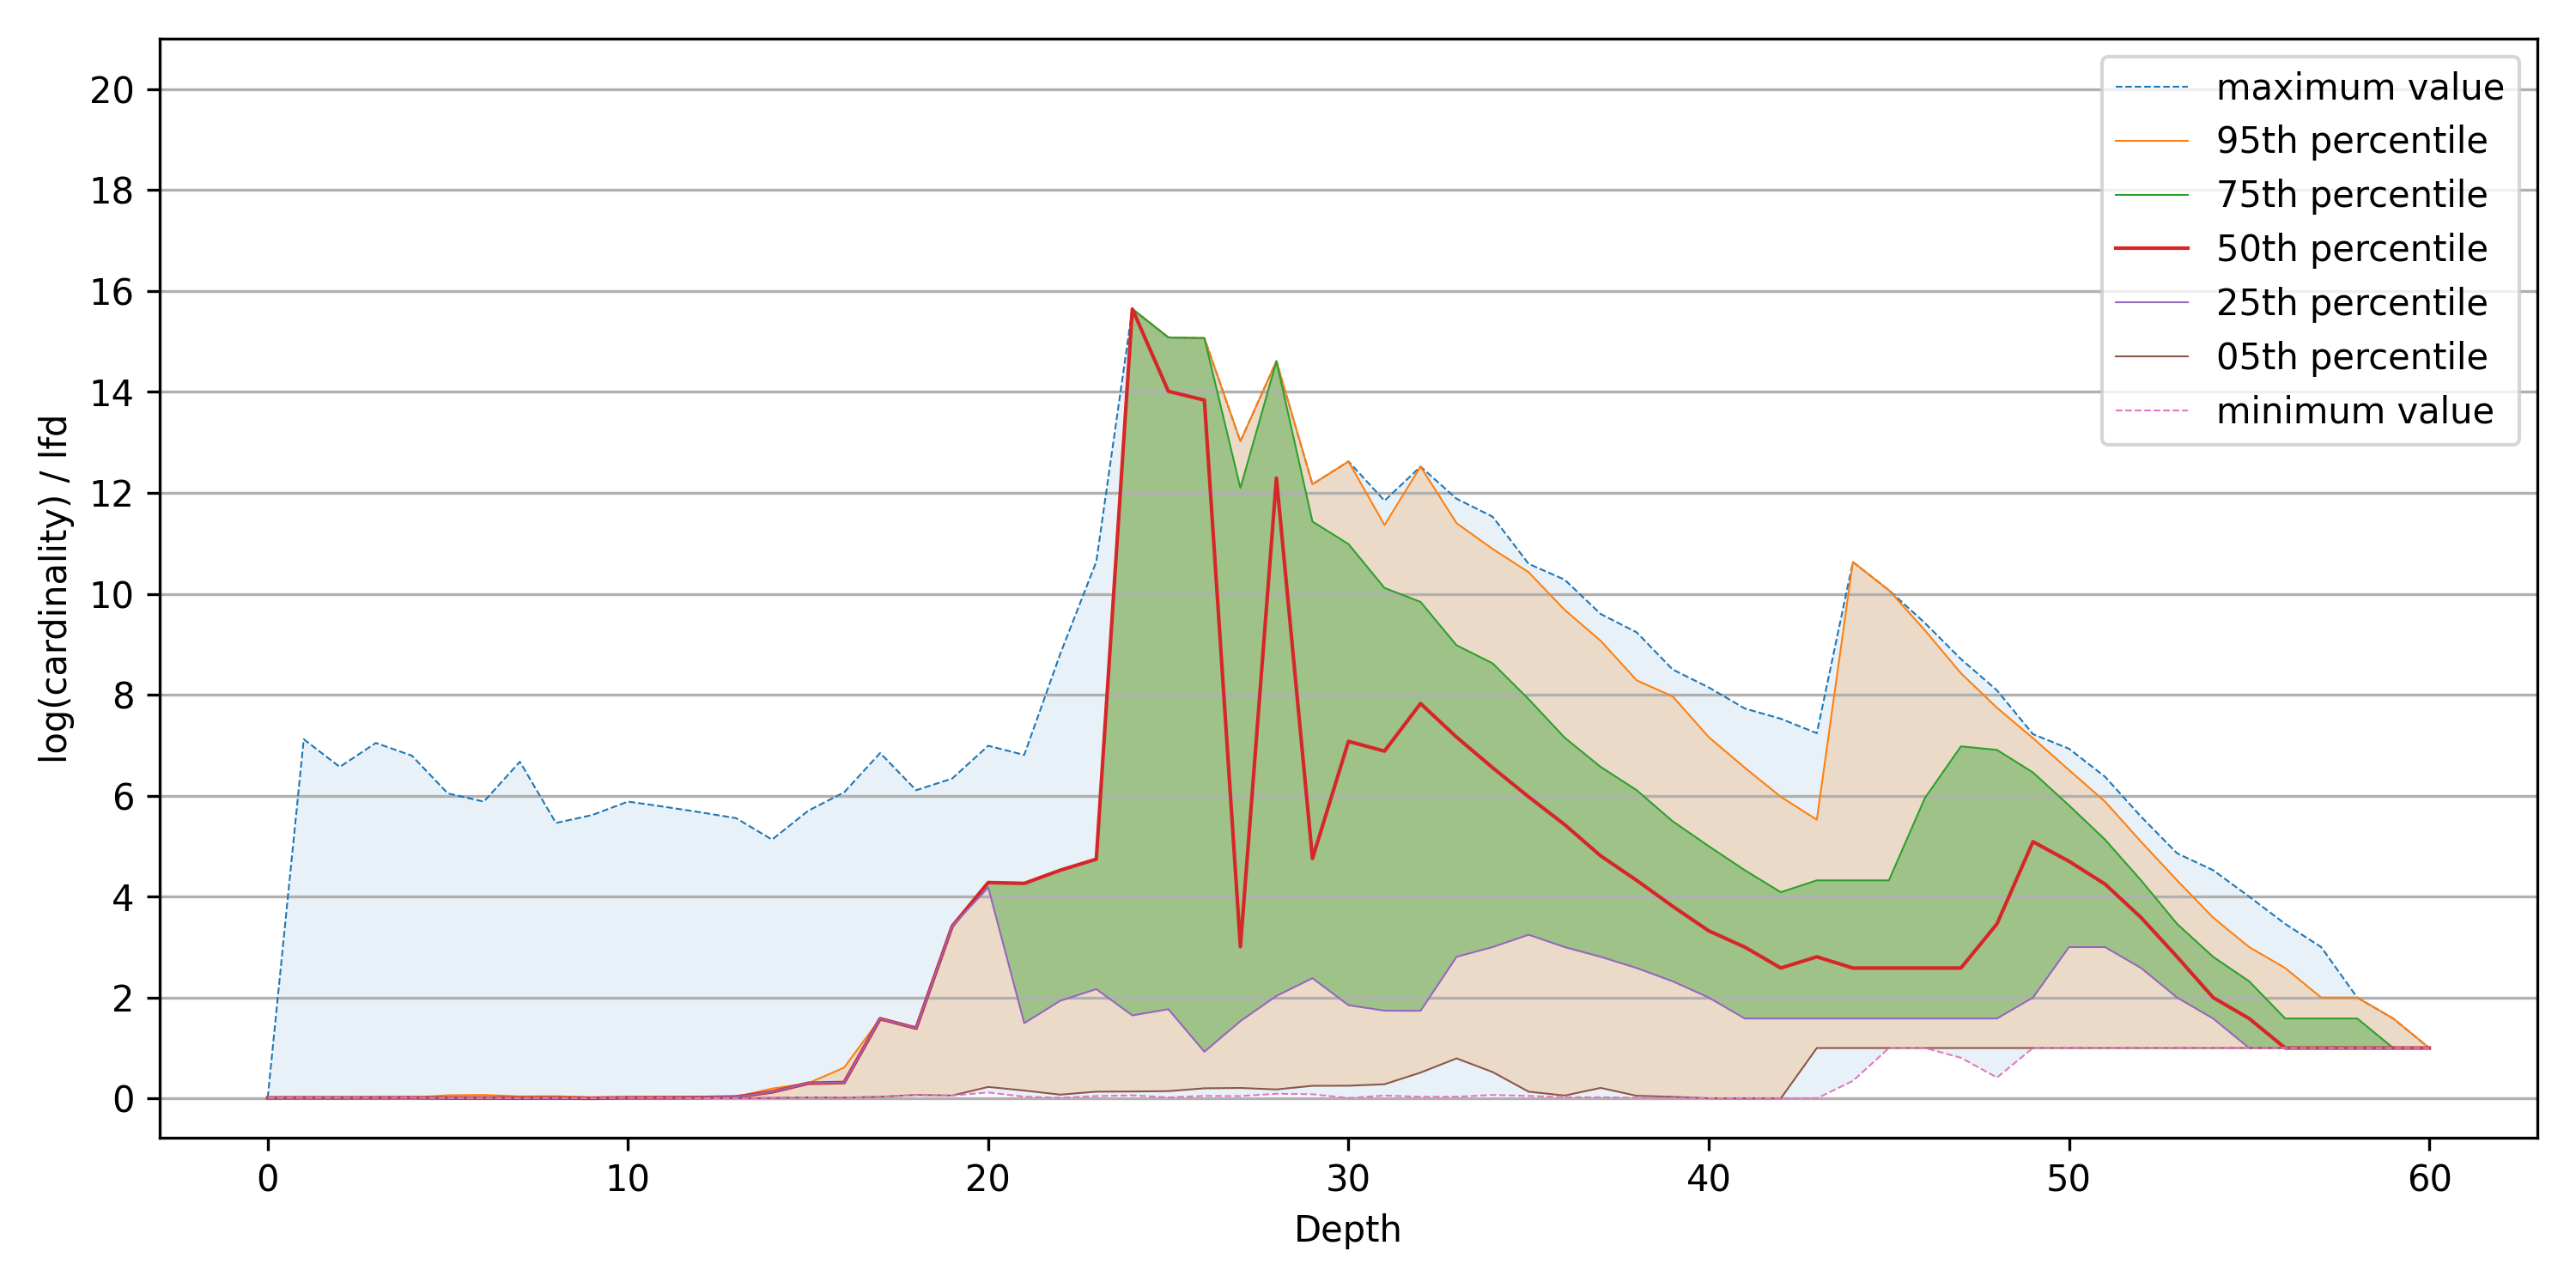
\includegraphics[width=0.95\textwidth]{images/lfd/radio-ml-97920.png}\\
        \subcaption{RadioML}
        \label{fig:results:radioml-lfd}
    \end{subfigure}%
    \begin{subfigure}[b]{0.47\textwidth}
        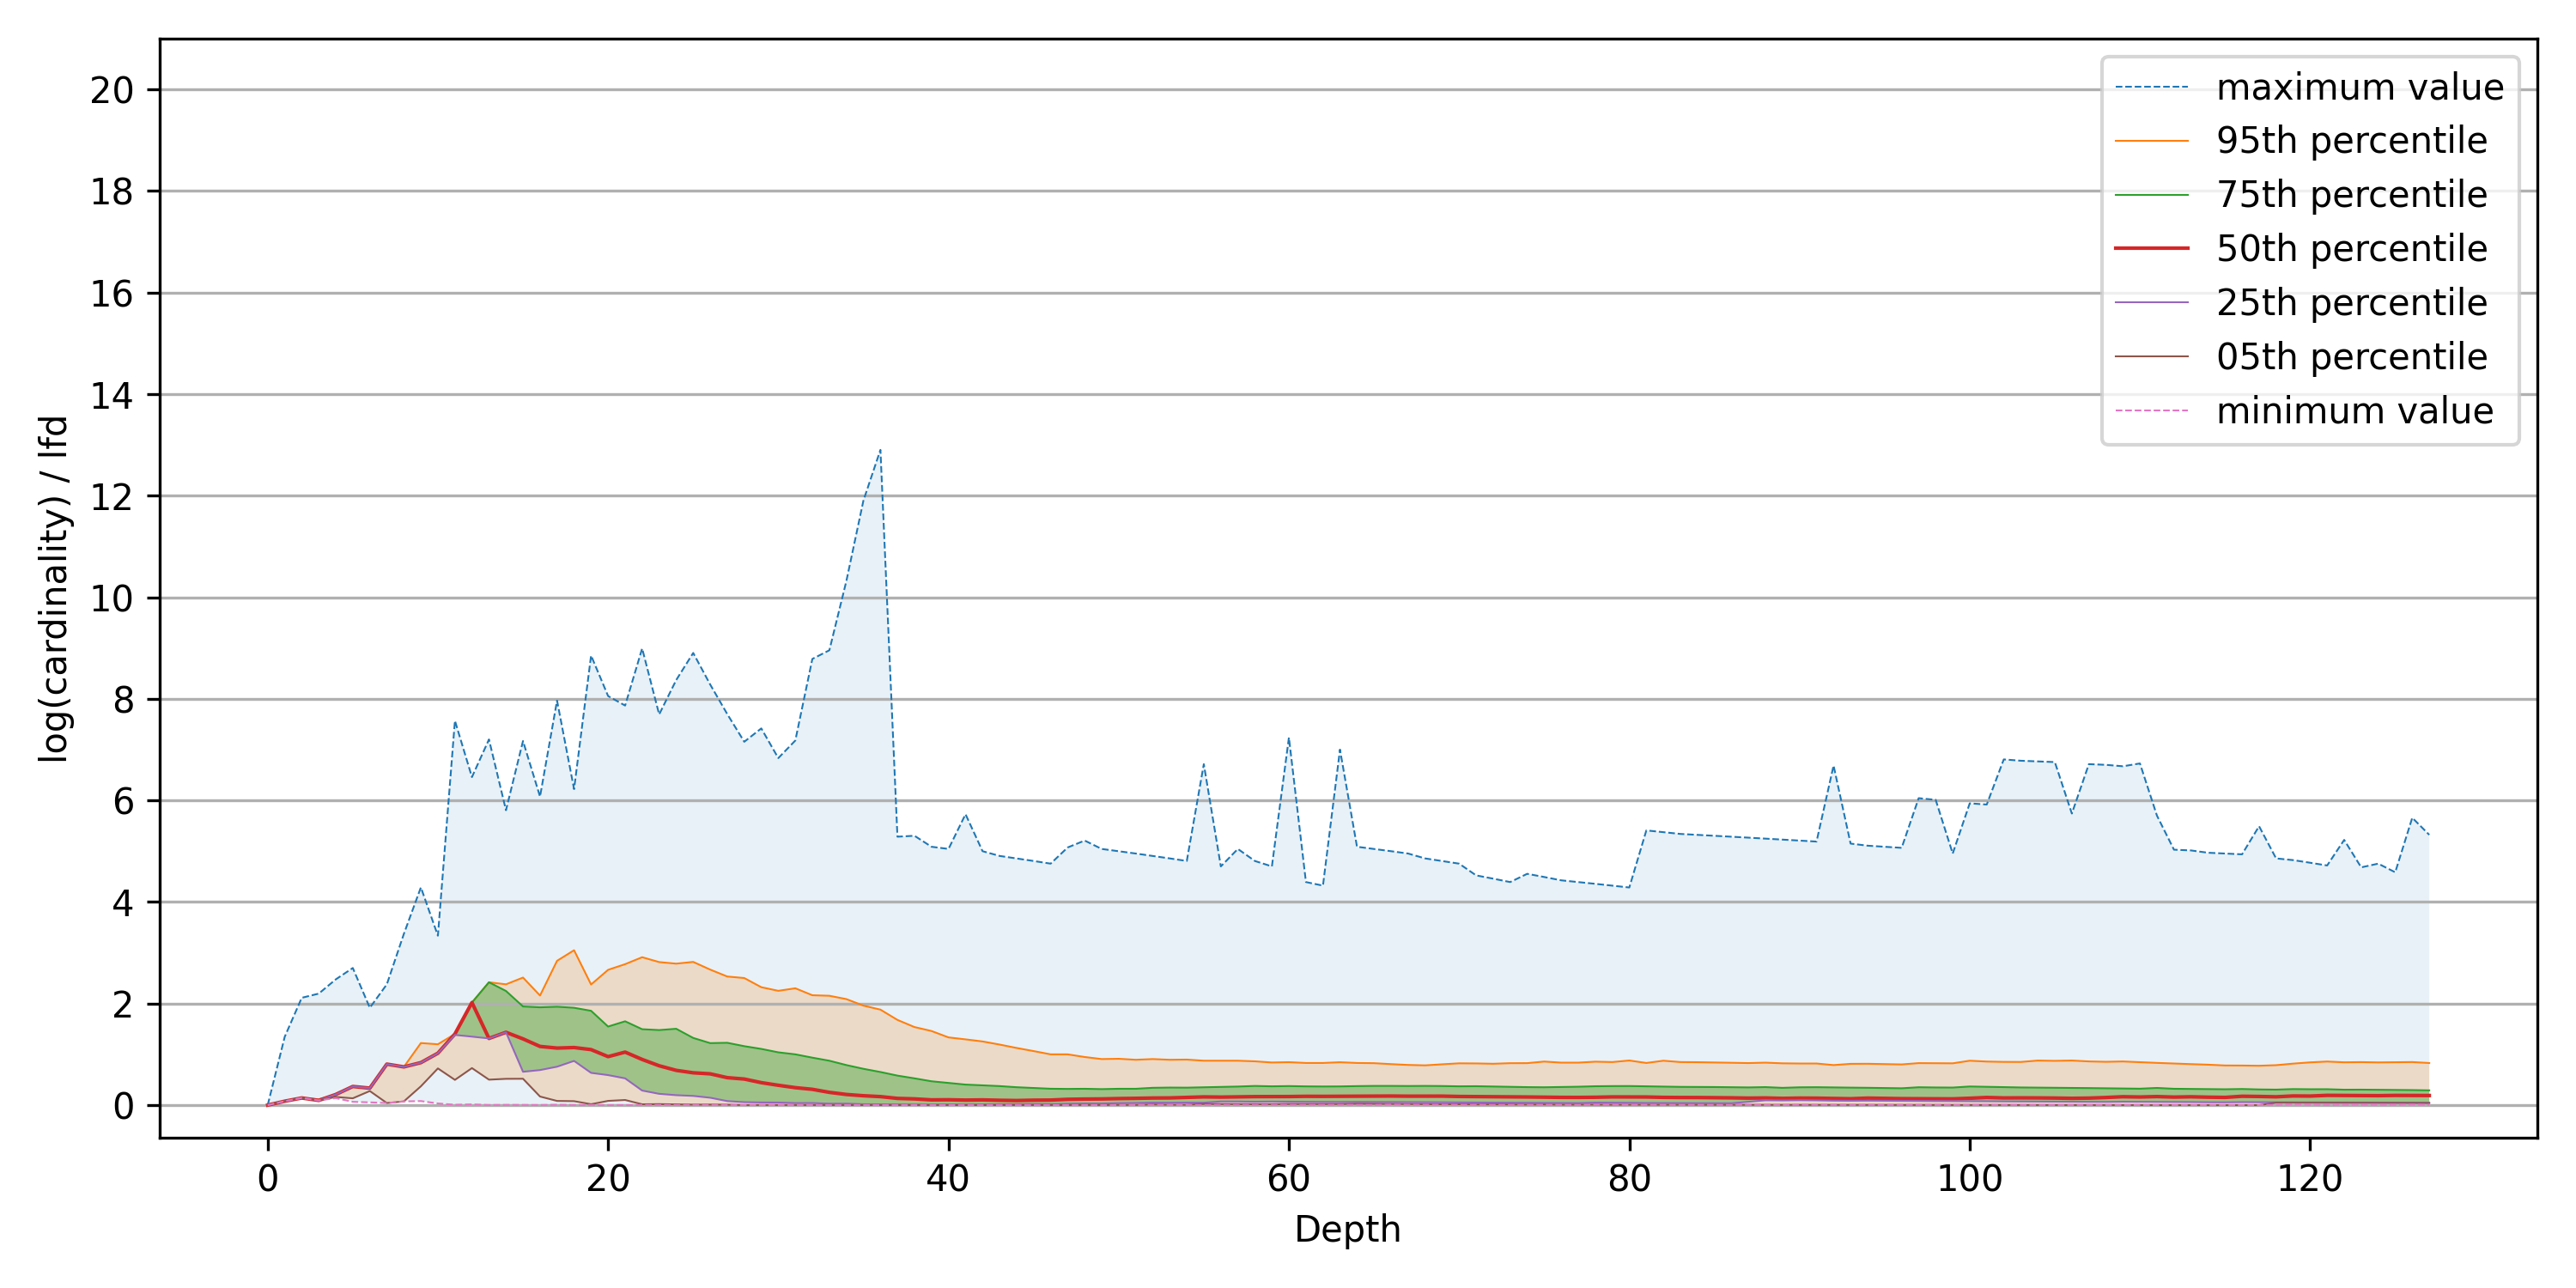
\includegraphics[width=0.95\textwidth]{images/lfd/silva-2224640.png}\\
        \subcaption{Silva 18S}
        \label{fig:results:silva-lfd}
    \end{subfigure}%
    \vspace{1em}
    \caption{Local fractal dimension vs. cluster depth across six datasets, grouped by decile of local fractal dimension and weighted by the cardinalities of the clusters.
    The last dataset is randomly generated.}
    \label{fig:results:lfd-plots}
\end{figure}


\subsection{Indexing and Tuning Time}
\label{sec:results:indexing-and-tuning-time}

For each of the ANN-benchmark datasets and the Random dataset, we report the time taken for each algorithm to build the index and to tune the hyper-parameters for these indices to achieve the highest possible recall. For the sake of brevity, these results are reported in the supplement.


\subsection{Scaling Behavior and Recall}
\label{sec:results:scaling-behavior-and-recall}

Figures~\ref{fig:results:fashion-mnist-scaling},~\ref{fig:results:glove-25-scaling},~and~\ref{fig:results:sift-scaling} show the scaling behavior of CAKES algorithms and existing algorithms on augmented versions of Fashion-Mnist under Euclidean distance,
Glove-25 under cosine distance, and
Sift under Euclidean distance.
Figure~\ref{fig:results:random-scaling} shows the scaling behavior of CAKES algorithms and existing algorithms on a completely randomly generated dataset with the same cardinality and dimensionality as Sift (1 million points in 128 dimensions).
Figures~\ref{fig:results:silva-scaling} and ~\ref{fig:results:radioml-scaling} show the scaling behavior of CAKES on Silva and RadioML respectively.
For these datasets, we took random sub-samples of the full datasets instead of augmenting them to higher cardinalities.
The horizontal axis in each figure shows the cardinality of the dataset augmented with synthetic points (see Section \ref{sec:methods:synthetic-data}).
The left-most point on each line is at the cardinality of the original dataset.
The vertical axis denotes throughput in queries per second.
Both axes are on a logarithmic scale.
In this section, we report results only for $k$-NN search with $k = 10$, but similar plots for $k = 100$ can be found in the Supplement.
For HNSW and ANNOY, we report the recall for each measurement in the plots. For algorithms which exhibit recall greater than $0.9995$, we do not report the recall in the plots, but we do report it in the tables below.

Table~\ref{tab:results:qps-and-recall} show the throughput and recall of CAKES's algorithms at each augmented cardinality for Fashion-Mnist, Glove-25, Sift, and Random.
Though the plots in Figure~\ref{fig:results:scaling-plots} present results for each of CAKES's three algorithms separately, the results in the CAKES column in these tables represent the fastest CAKES algorithm at that dataset and cardinality only.
We used our auto-tuning approach (see Section~\ref{sec:methods:auto-tuning}) for each new tree (i.e.,\,at each cardinality), and this approach was always able to select the fastest algorithm for each dataset at each cardinality.
Since we also allow for tuning hyper-parameters for the other algorithms, and we allow for different sets of hyper-parameters at each cardinality, it is a fair comparison for these tables to only list the performance of the tuned CAKES algorithm.
When reporting recall, we use $1.000*$ to denote that the recall is imperfect, but rounds to $1.000$.


Figure~\ref{fig:results:scaling-plots} shows that for Fashion-Mnist, Glove-25, and Sift, as cardinality increases, the CAKES algorithms (Depth-First Sieve in blue, Repeated $\rho$-NN in green, and Breadth-First Sieve in purple) become faster than our Rust implementation of na\"{i}ve linear search (in orange).
Though we observe this trend, we note that the exact cardinality at which CAKES's algorithms overtake linear search differs by dataset. For Fashion-Mnist, CAKES begins outperforming linear search starting at a cardinality near $10^5$, while for Glove-25 and Sift, this happens near $10^6$ and $10^7$ respectively.
Which one of the three CAKES algorithms is fastest also differs by dataset.
For Fashion-Mnist, Depth-First Sieve is consistently fastest, while for Glove-25, the fastest is Repeated $\rho$-NN, and for Sift, Breadth-First Sieve.
On all three datasets, Depth-First Sieve and Breadth-First Sieve appear to have performance which is \textit{constant} in the cardinality of the dataset.
With Glove-25, Repeated $\rho$-NN exhibits similar constant scaling.
We also observe that on these three datasets, for nearly all cardinalities, all three of the CAKES algorithms are faster than FAISS-Flat (in brown), and that at some cardinality, CAKES's algorithms become faster than FAISS-IVF (in pink).
For Fashion-Mnist, CAKES becomes faster than FAISS-IVF near cardinality $10^5$, whereas for Glove-25 and Sift, this happens near cardinality $10^7$.
On all three of these datasets, HNSW (in gray) and ANNOY (in yellow) are faster than CAKES's algorithms for all cardinalities; however, CAKES exhibits perfect or near-perfect recall on each dataset, while HNSW and ANNOY exhibit much lower recall, as shown in Table~\ref{tab:datasets:summary}.
While recall for CAKES's does \emph{not} degrade with cardinality, recall for HNSW and ANNOY degrades with cardinality.
At a cardinality multiplier as low as eight, HNSW and ANNOY have recall of $0.525$ and $0.857$ respectively for Fashion-Mnist, 0.607 and 0.832 for Glove-25, and 0.782 and 0.686 on Sift.
In contrast, CAKES has perfect recall on Fashion-Mnist and Sift (where the distance function is a metric), and near-perfect recall on Glove-25 (cosine distance is not a metric).


In contrast with the results on the ANN Benchmark datasets reported above, with the Random dataset, as seen in Figure~\ref{fig:results:random-scaling}, we observe performs quite slowly.
As with the real datasets, HNSW and ANNOY are the fastest algorithms, and CAKES exhibits perfect recall at all cardinalities.
HNSW and ANNOY exhibit \textit{much} lower recall on this random dataset than on any of the ANN benchmark datasets;
in particular, with a multiplier of 1, HNSW and ANNOY have recall as low as 0.060 and 0.028 respectively, as reported in Tables~\ref{tab:results:qps-and-recall-fmn},~\ref{tab:results:qps-and-recall-glove},~\ref{tab:results:qps-and-recall-sift}, and~\ref{tab:results:qps-and-recall-random}.

For Silva and RadioML, we benchmarked only CAKES's algorithms because HNSW, ANNOY and FAISS support neither the required distance functions nor, in the case of RadioML, complex-valued data.
Due to the massive sizes of these datasets and challenges in generating plausible augmentations, we took random sub-samples ranging up to the entirety of the dataset---rather than augmented versions of the dataset---to examine how performance scales with cardinality.
With Silva, as shown in Figure~\ref{fig:results:silva-scaling}, we observe that for all algorithms, throughput initially seems to linearly decrease as cardinality increases, but that it seems to begin levelling off near cardinality $10^5$.
Until cardinality near $10^4$, Depth-First Sieve is the fastest CAKES algorithm, but for larger cardinalities, Repeated $\rho$-NN is the fastest CAKES algorithm.
For RadioML, as shown in Figure~\ref{fig:results:radioml-scaling}, we observe that throughput declines nearly linearly, and that the three CAKES algorithms exhibit virtually indistinguishable performance.
In particular, throughput of CAKES's algorithms is identical within three significant figures.

\begin{figure}
    \begin{subfigure}[b]{0.47\textwidth}
        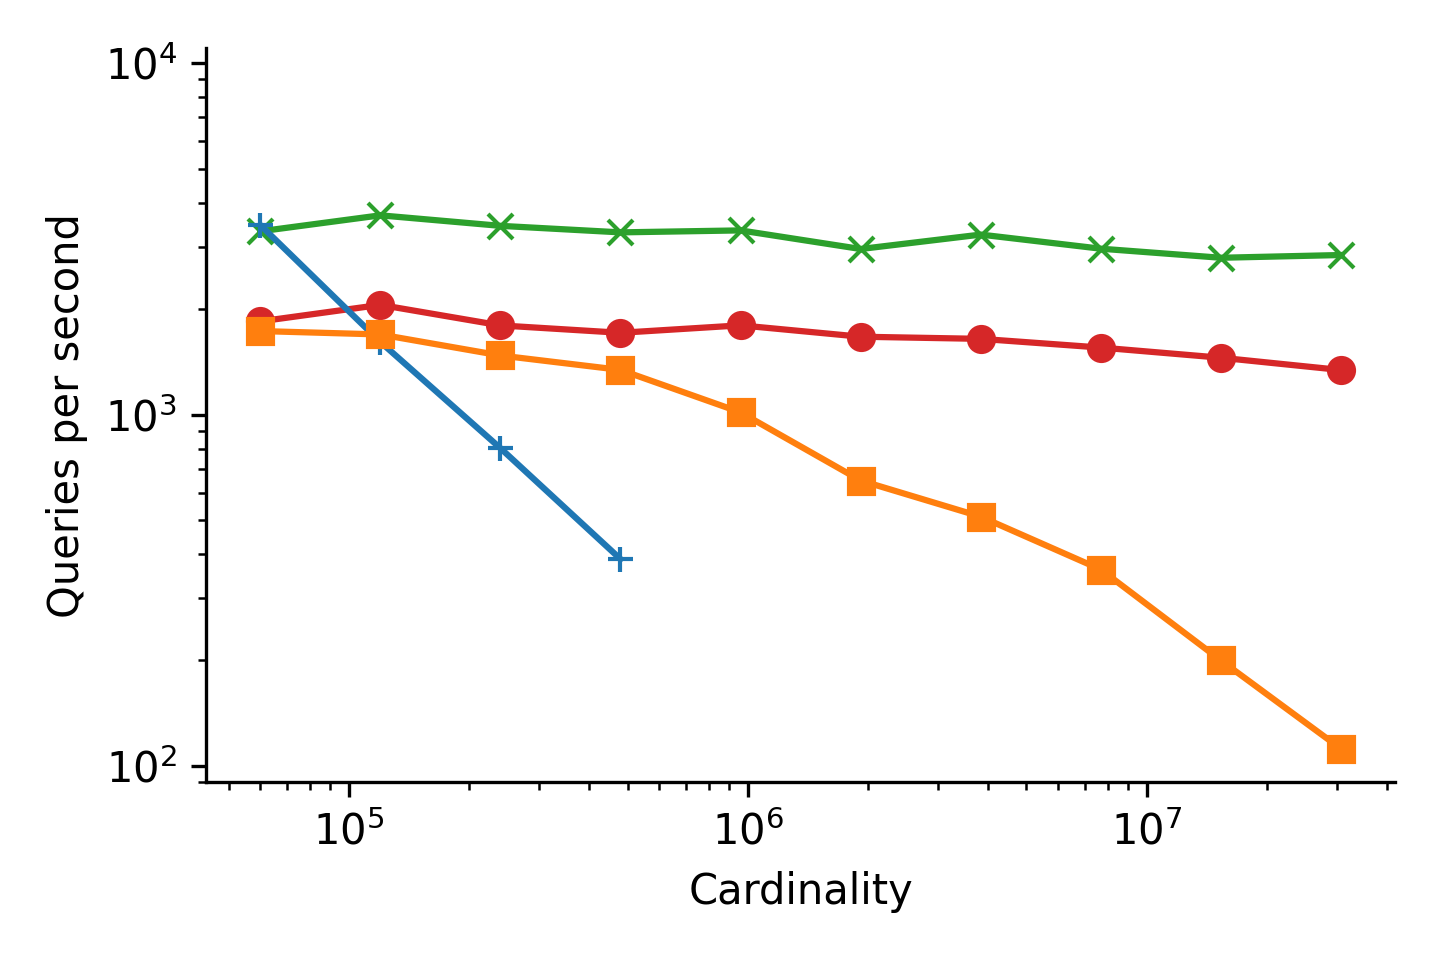
\includegraphics[width=0.95\textwidth]{plots/fashion-mnist_PermutedBall_10_throughput.png}
        \subcaption{Fashion-Mnist for $k=10$.}
        \label{fig:results:fashion-mnist-scaling}
    \end{subfigure}%
    \begin{subfigure}[b]{0.47\textwidth}
        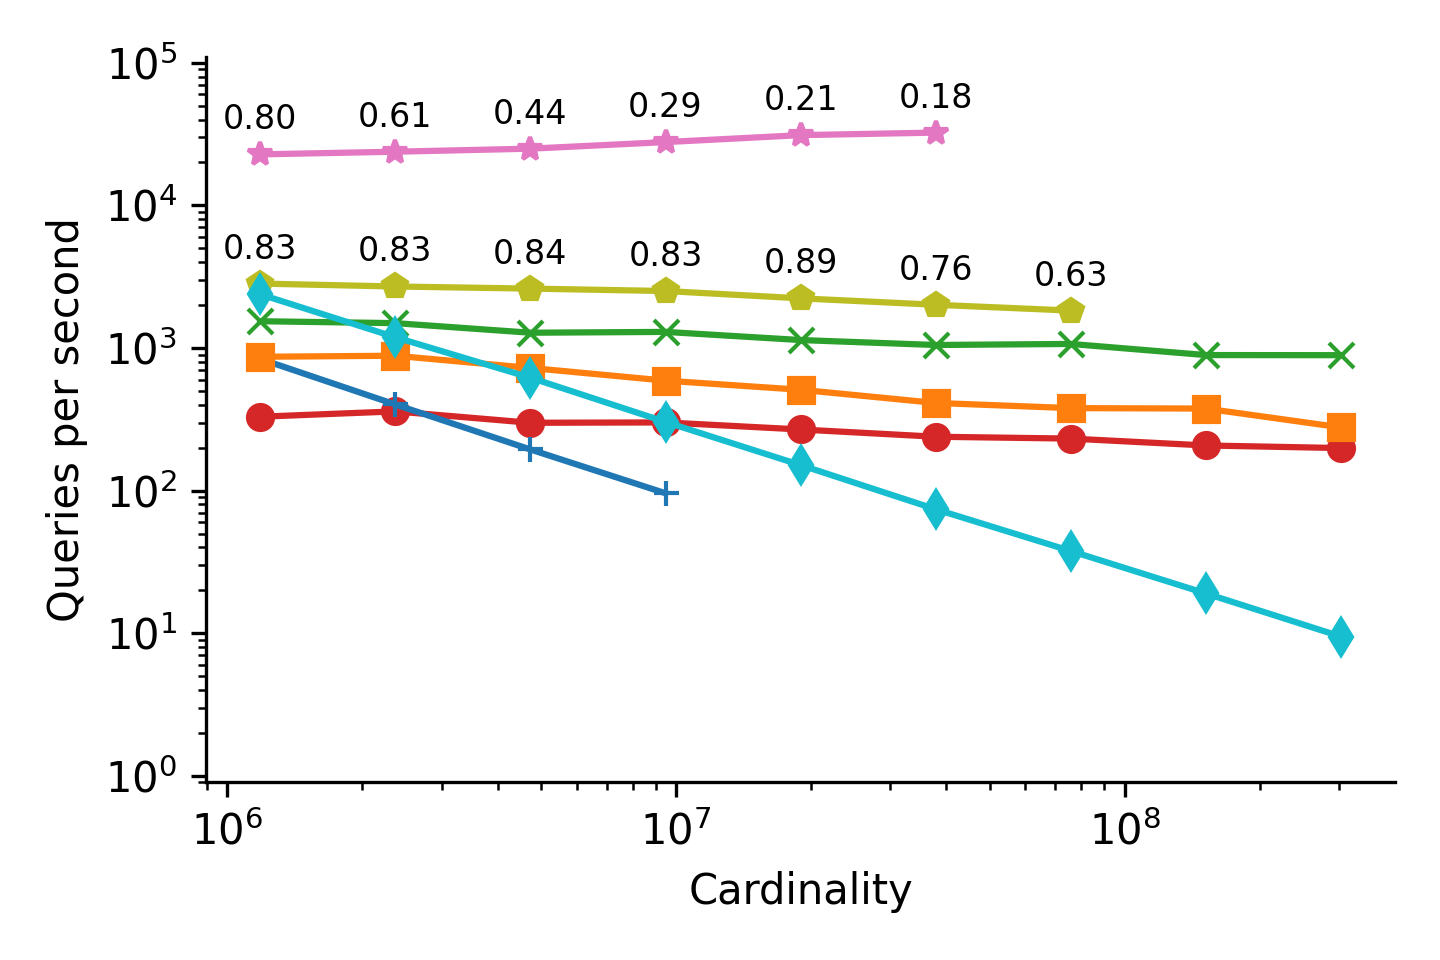
\includegraphics[width=0.95\textwidth]{plots/glove-25_PermutedBall_10_throughput.png}
        \subcaption{Glove-25 for $k=10$.}
        \label{fig:results:glove-25-scaling}
    \end{subfigure}%
    \vspace{1em}
    \\
    \begin{subfigure}[b]{0.47\textwidth}
        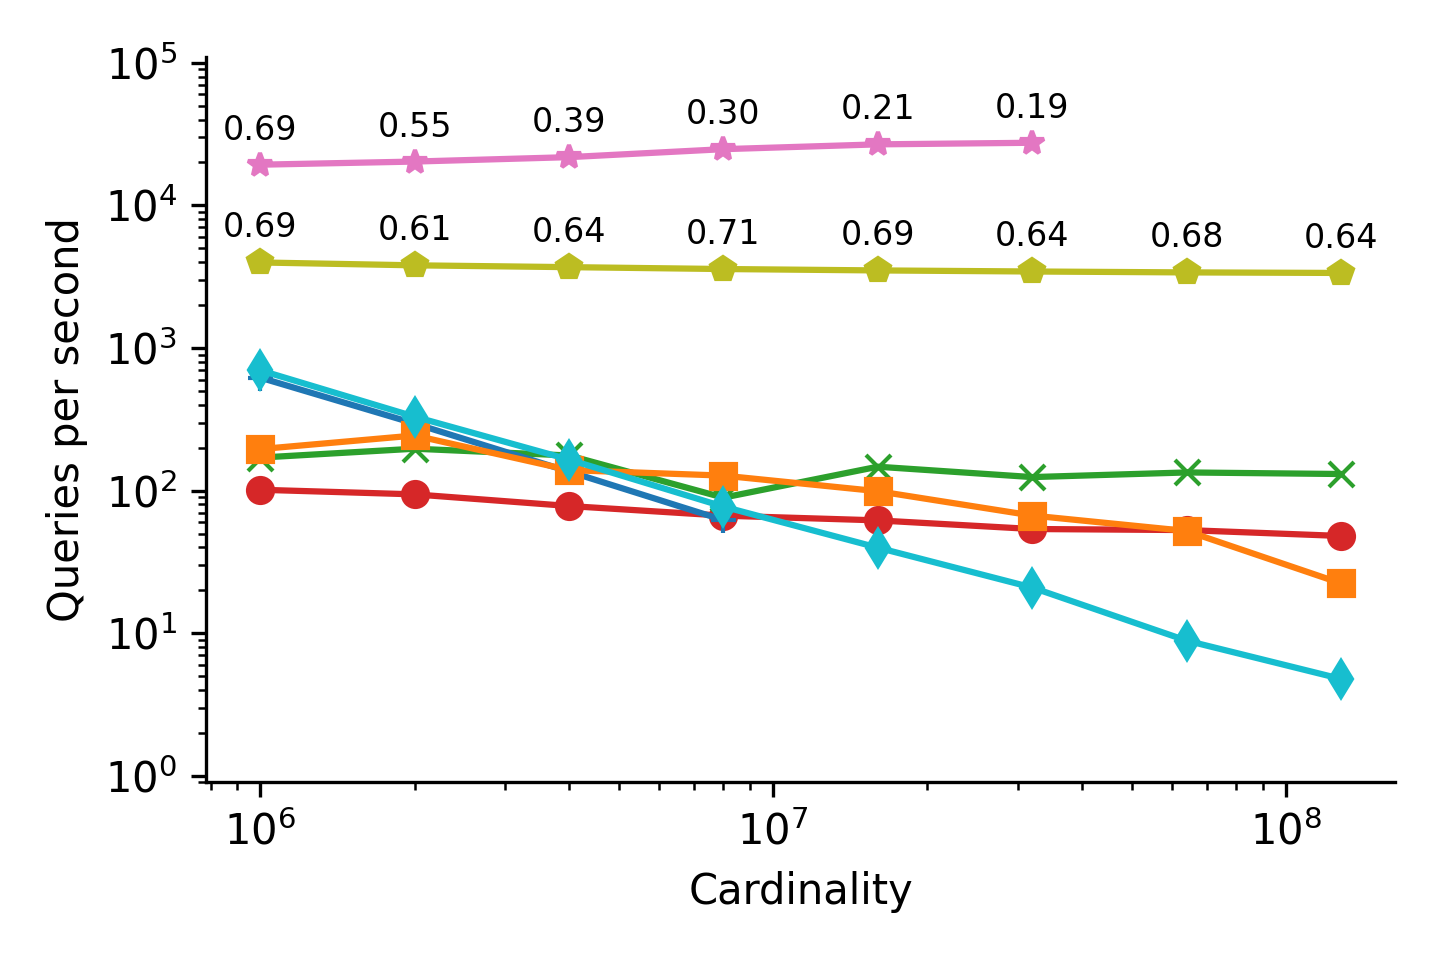
\includegraphics[width=0.95\textwidth]{plots/sift_PermutedBall_10_throughput.png}
        \subcaption{Sift for $k=10$.}
        \label{fig:results:sift-scaling}
    \end{subfigure}%
    \begin{subfigure}[b]{0.47\textwidth}
        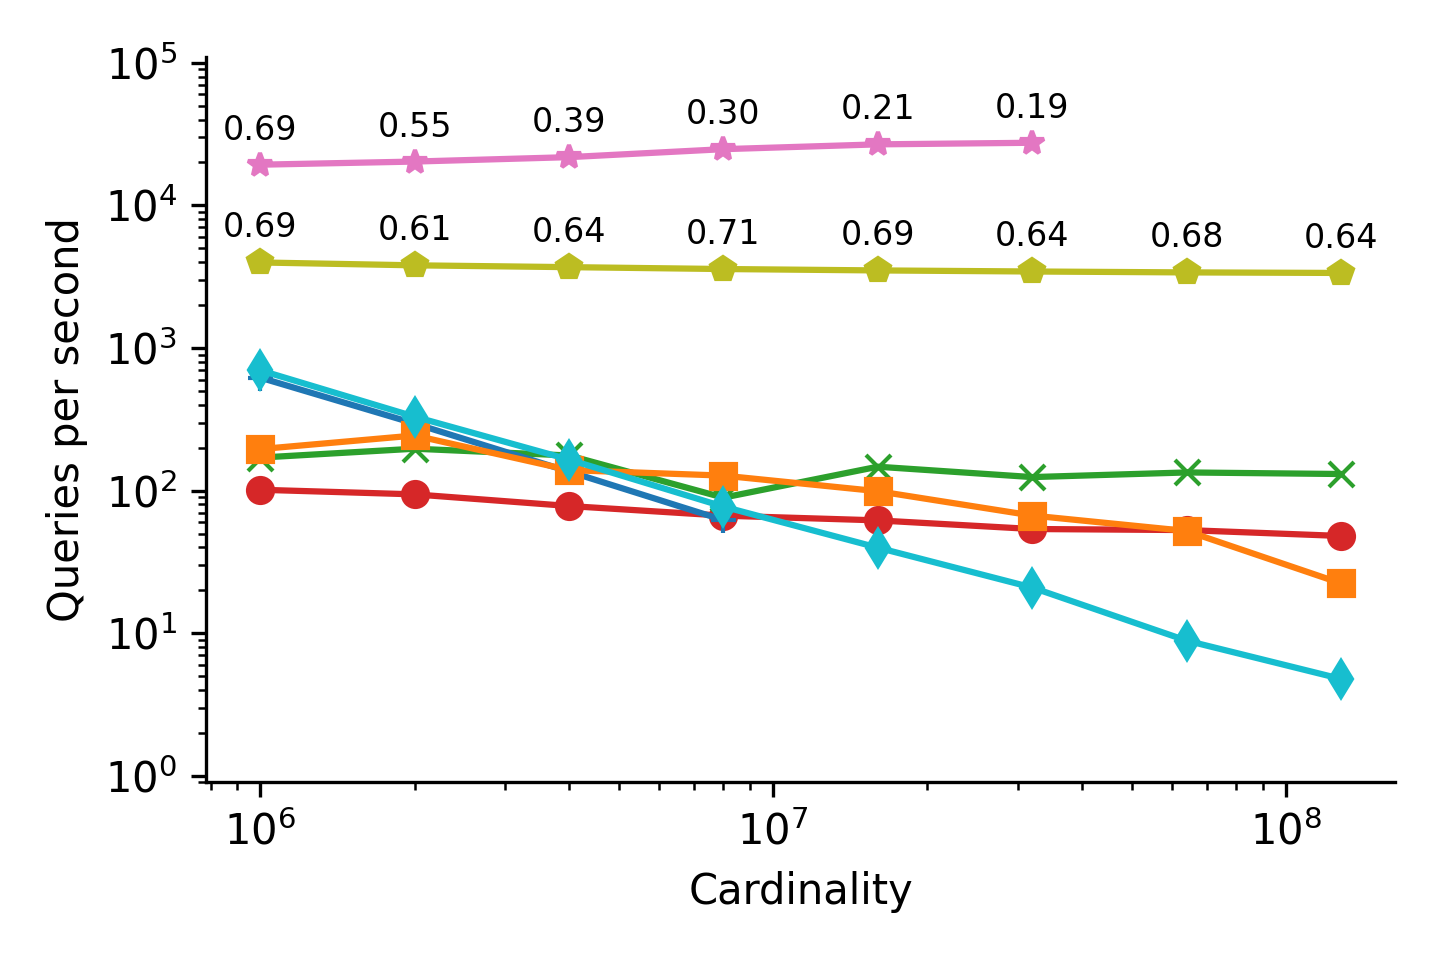
\includegraphics[width=0.95\textwidth]{plots/sift_PermutedBall_10_throughput.png}
        \subcaption{A random dataset for $k=10$.}
        \label{fig:results:random-scaling}
    \end{subfigure}%
    \\
    \begin{subfigure}[b]{0.47\textwidth}
        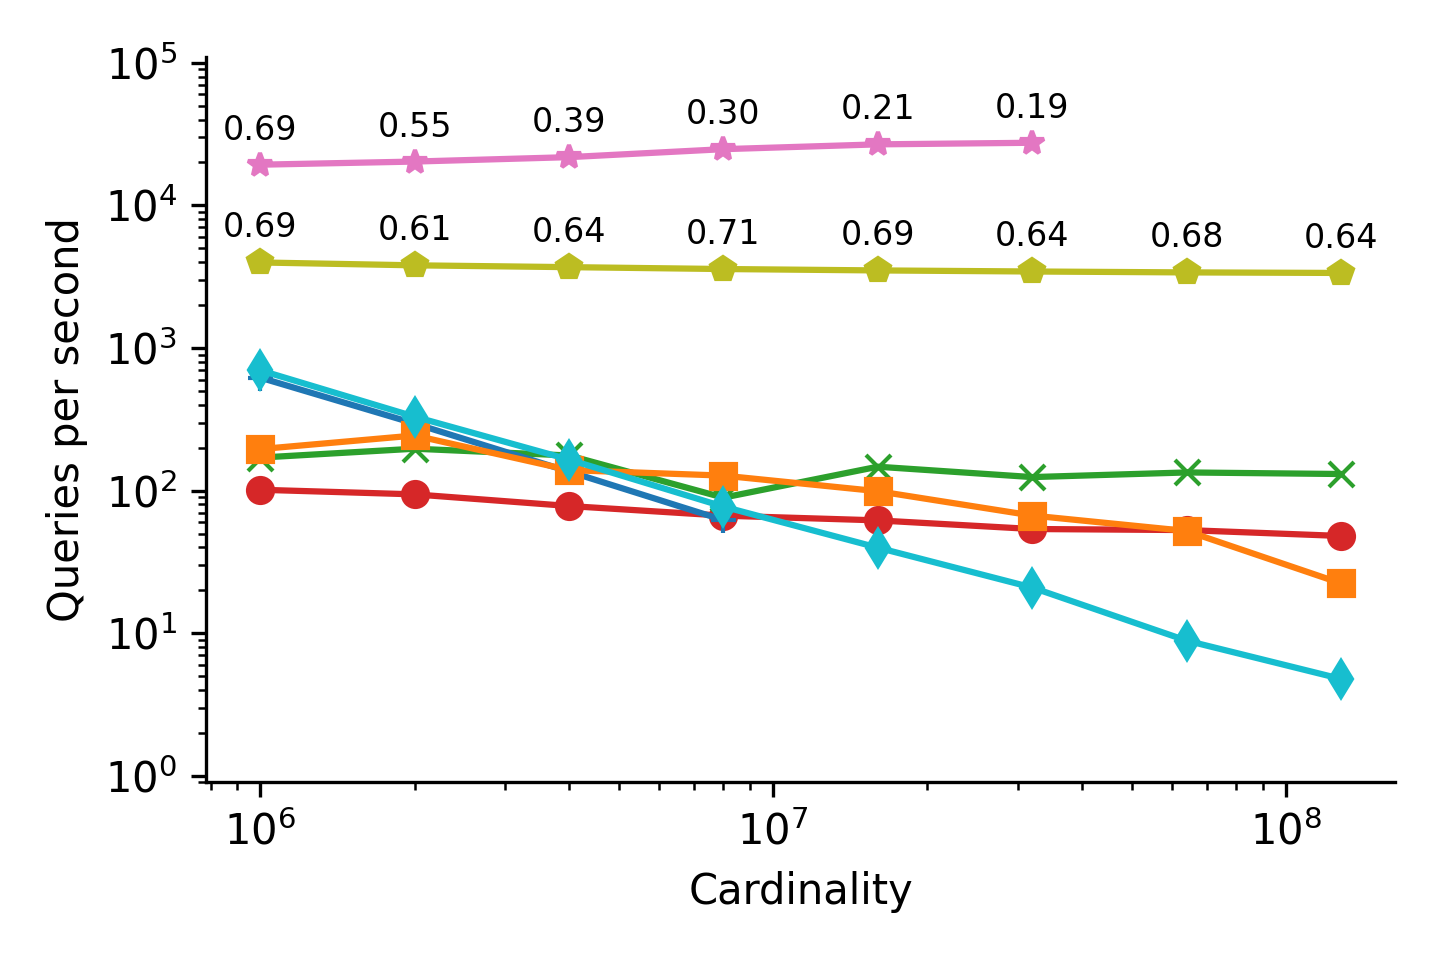
\includegraphics[width=0.95\textwidth]{plots/sift_PermutedBall_10_throughput.png}
        \subcaption{RadioML for $k=10$ at SnR = 10dB.}
        \label{fig:results:radioml-scaling}
    \end{subfigure}%
    \vspace{1em}
    \begin{subfigure}[b]{0.47\textwidth}
        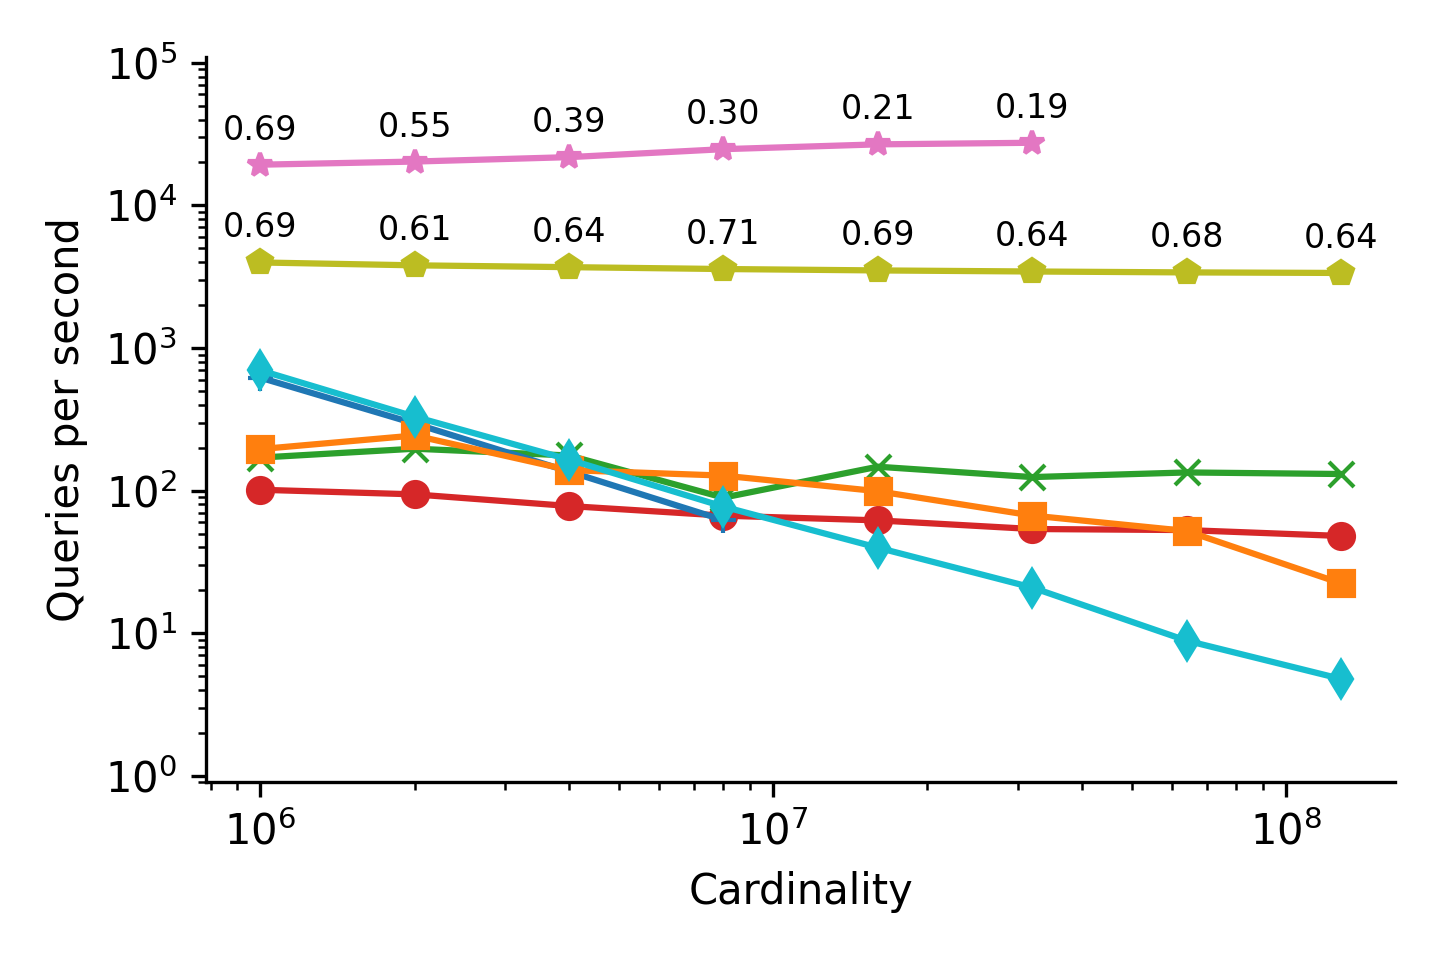
\includegraphics[width=0.95\textwidth]{plots/sift_PermutedBall_10_throughput.png}
        \subcaption{Silva for $k=10$.}
        \label{fig:results:silva-scaling}
    \end{subfigure}%
    \caption{Throughput across six datasets, including a randomly-generated dataset.
    In each plot, the horizontal axis represents increasing cardinality of the dataset, while the vertical axis represents the throughput in queries per second (higher is better).
    Note that for RadioML, all three algorithms performed nearly identically, so distinct lines are not visible.
    For some algorithms, we were not able to take measurements for each cardinality because the index-building required more RAM than was available (i.e.,\,more then 512GB).
    For linear search with CAKES, we only report the throughput for a few of the initial multipliers because the trend is clear.}
    \label{fig:results:scaling-plots}
\end{figure}


\begin{table*}[h]
    % \renewcommand{\arraystretch}{1.15}
    \caption{Queries per second (QPS) and Recall vs naive linear search on the Fashion-Mnist dataset.
    A recall value of $1.000*$ denotes imperfect recall that rounds to 1.000.}
    \label{tab:results:qps-and-recall-fmn}
    \vskip 0.15in
    \begin{center}
        %\begin{small}
            \begin{tabular}{|c|l|p{1.4cm}|p{1.0cm}|p{1.4cm}|p{1.0cm}|p{1.4cm}|p{1.0cm}|p{1.4cm}|p{1.0cm}|}
                \hline
                & \multirow{2}{*}{\textbf{Mult.}} & \multicolumn{2}{|c}{\textbf{hnsw}} & \multicolumn{2}{|c}{\textbf{annoy}} & \multicolumn{2}{|c}{\textbf{faiss-ivf}}  & \multicolumn{2}{|c|}{\textbf{cakes}} \\\cline{3-10}
                & & QPS & Recall & QPS & Recall & QPS & Recall & QPS & Recall \\
                \cline{2-10}
                \hline
                \multirow{10}{*}{\rotatebox[origin=c]{90}{\textbf{Fashion-Mnist}}}
                & 1   & \num{1.33e4} & 0.954  & \num{2.19e3} & 0.950  & \num{2.01e3} & 1.000* & \num{3.46e3} & 1.000  \\\cline{2-10}
                & 2   & \num{1.38e4} & 0.803  & \num{2.12e3} & 0.927  & \num{9.39e2} & 1.000* & \num{3.68e3} & 1.000  \\\cline{2-10}
                & 4   & \num{1.66e4} & 0.681  & \num{2.04e3} & 0.898  & \num{4.61e2} & 0.997  & \num{3.44e3} & 1.000  \\\cline{2-10}
                & 8   & \num{1.68e4} & 0.525  & \num{1.93e3} & 0.857  & \num{2.26e2} & 0.995  & \num{3.30e3} & 1.000  \\\cline{2-10}
                & 16  & \num{1.87e4} & 0.494  & \num{1.84e3} & 0.862  & \num{1.17e2} & 0.991  & \num{3.34e3} & 1.000  \\\cline{2-10}
                & 32  & \num{1.56e4} & 0.542  & \num{1.85e3} & 0.775  & \num{5.91e1} & 0.985  & \num{2.96e3} & 1.000  \\\cline{2-10}
                & 64  & \num{1.50e4} & 0.378  & \num{1.78e3} & 0.677  & \num{2.61e1} & 0.968  & \num{3.25e3} & 1.000  \\\cline{2-10}
                & 128 & \num{1.49e4} & 0.357  & \num{1.66e3} & 0.538  & \num{1.33e1} & 0.964  & \num{2.96e3} & 1.000  \\\cline{2-10}
                & 256 & --           & --     & \num{1.60e3} & 0.592  & \num{6.65e0} & 0.962  & \num{2.79e3} & 1.000  \\\cline{2-10}
                & 512 & --           & --     & \num{1.83e3} & 0.581  & \num{3.56e0} & 0.949 & \num{2.84e3} & 1.000 \\
                \hline
            \end{tabular}
        %\end{small}
    \end{center}
    \vskip -0.1in
\end{table*}


\begin{table*}[h]
    % \renewcommand{\arraystretch}{1.15}
    \caption{Queries per second (QPS) and Recall vs naive linear search on the Glove-25 dataset.
    A recall value of $1.000*$ denotes imperfect recall that rounds to 1.000.}
    \label{tab:results:qps-and-recall-glove}
    \vskip 0.15in
    \begin{center}
        \begin{small}
            \begin{tabular}{|c|l|p{1.4cm}|p{1.0cm}|p{1.4cm}|p{1.0cm}|p{1.4cm}|p{1.0cm}|p{1.4cm}|p{1.0cm}|}
                \hline
                & \multirow{2}{*}{\textbf{Mult.}} & \multicolumn{2}{|c}{\textbf{hnsw}} & \multicolumn{2}{|c}{\textbf{annoy}} & \multicolumn{2}{|c}{\textbf{faiss-ivf}}  & \multicolumn{2}{|c|}{\textbf{cakes}} \\\cline{3-10}
                & & QPS & Recall & QPS & Recall & QPS & Recall & QPS & Recall \\
                \cline{2-10}

                \hline
                \multirow{9}{*}{\rotatebox[origin=c]{90}{\textbf{Glove-25}}}
                & 1   & \num{2.28e4} & 0.801 & \num{2.83e3} & 0.835 & \num{2.38e3} & 1.000* & \num{1.54e3} & 1.000* \\\cline{2-10}
                & 2   & \num{2.38e4} & 0.607 & \num{2.70e3} & 0.832 & \num{1.19e3} & 1.000* & \num{1.49e3} & 1.000* \\\cline{2-10}
                & 4   & \num{2.50e4} & 0.443 & \num{2.61e3} & 0.839 & \num{6.19e2} & 1.000* & \num{1.28e3} & 1.000* \\\cline{2-10}
                & 8   & \num{2.78e4} & 0.294 & \num{2.51e3} & 0.834 & \num{3.03e2} & 1.000* & \num{1.30e3} & 1.000* \\\cline{2-10}
                & 16  & \num{3.11e4} & 0.213 & \num{2.23e3} & 0.885 & \num{1.51e2} & 1.000* & \num{1.14e3} & 1.000* \\\cline{2-10}
                & 32  & \num{3.24e4} & 0.178 & \num{2.01e3} & 0.764 & \num{7.40e1} & 0.999  & \num{1.05e3} & 1.000* \\\cline{2-10}
                & 64  & --           & --    & \num{1.99e3} & 0.631 & \num{3.77e1} & 0.997  & \num{1.07e3} & 1.000* \\\cline{2-10}
                & 128 & --           & --    & --           & --    & \num{1.90e1} & 0.998  & \num{8.92e2} & 1.000* \\\cline{2-10}
                & 256 & --           & --    & --           & --    & \num{9.47e0} & 0.998  & \num{8.91e2} & 1.000* \\
                \hline

            \end{tabular}
        \end{small}
    \end{center}
    \vskip -0.1in
\end{table*}


\begin{table*}[h]
    % \renewcommand{\arraystretch}{1.15}
    \caption{Queries per second (QPS) and Recall vs naive linear search on the Sift dataset.
    A recall value of $1.000*$ denotes imperfect recall that rounds to 1.000.}
    \label{tab:results:qps-and-recall-sift}
    \vskip 0.15in
    \begin{center}
        \begin{small}
            \begin{tabular}{|c|l|p{1.4cm}|p{1.0cm}|p{1.4cm}|p{1.0cm}|p{1.4cm}|p{1.0cm}|p{1.4cm}|p{1.0cm}|}
                \hline
                & \multirow{2}{*}{\textbf{Mult.}} & \multicolumn{2}{|c}{\textbf{hnsw}} & \multicolumn{2}{|c}{\textbf{annoy}} & \multicolumn{2}{|c}{\textbf{faiss-ivf}}  & \multicolumn{2}{|c|}{\textbf{cakes}} \\\cline{3-10}
                & & QPS & Recall & QPS & Recall & QPS & Recall & QPS & Recall \\
                \cline{2-10}

                \hline
                \multirow{8}{*}{\rotatebox[origin=c]{90}{\textbf{Sift}}}
                & 1   & \num{1.93e4} & 0.782 & \num{3.98e3} & 0.686 & \num{6.98e2} & 1.000* & \num{6.20e2} & 1.000 \\\cline{2-10}
                & 2   & \num{2.03e4} & 0.552 & \num{3.80e3} & 0.614 & \num{3.30e2} & 1.000* & \num{2.95e2} & 1.000 \\\cline{2-10}
                & 4   & \num{2.18e4} & 0.394 & \num{3.69e3} & 0.637 & \num{1.65e2} & 1.000* & \num{1.76e2} & 1.000 \\\cline{2-10}
                & 8   & \num{2.48e4} & 0.298 & \num{3.58e3} & 0.710 & \num{7.72e1} & 1.000* & \num{1.27e2} & 1.000 \\\cline{2-10}
                & 16  & \num{2.68e4} & 0.210 & \num{3.50e3} & 0.690 & \num{3.98e1} & 1.000* & \num{1.47e2} & 1.000 \\\cline{2-10}
                & 32  & \num{2.75e4} & 0.193 & \num{3.44e3} & 0.639 & \num{2.09e1} & 0.999  & \num{1.24e2} & 1.000 \\\cline{2-10}
                & 64  & --           & --    & \num{3.39e3} & 0.678 & \num{8.87e0} & 0.997  & \num{1.34e2} & 1.000 \\\cline{2-10}
                & 128 & --           & --    & \num{3.36e3} & 0.643 & \num{4.78e0} & 0.993  & \num{1.31e2} & 1.000 \\
                \hline

            \end{tabular}
        \end{small}
    \end{center}
    \vskip -0.1in
\end{table*}

\begin{table*}[h]
    % \renewcommand{\arraystretch}{1.15}
    \caption{Queries per second (QPS) and Recall vs naive linear search on the Random dataset.
    A recall value of $1.000*$ denotes imperfect recall that rounds to 1.000.}
    \label{tab:results:qps-and-recall-random}
    \vskip 0.15in
    \begin{center}
        \begin{small}
            \begin{tabular}{|c|l|p{1.4cm}|p{1.0cm}|p{1.4cm}|p{1.0cm}|p{1.4cm}|p{1.0cm}|p{1.4cm}|p{1.0cm}|}
                \hline
                & \multirow{2}{*}{\textbf{Mult.}} & \multicolumn{2}{|c}{\textbf{hnsw}} & \multicolumn{2}{|c}{\textbf{annoy}} & \multicolumn{2}{|c}{\textbf{faiss-ivf}}  & \multicolumn{2}{|c|}{\textbf{cakes}} \\\cline{3-10}
                & & QPS & Recall & QPS & Recall & QPS & Recall & QPS & Recall \\
                \cline{2-10}

                \hline
                \multirow{6}{*}{\rotatebox[origin=c]{90}{\textbf{Random}}}
                & 1  & \num{1.17e4} & 0.060 & \num{4.28e3} & 0.028 & \num{7.342} & 1.000* & \num{5.54e2} & 1.000 \\\cline{2-10}
                & 2  & \num{1.01e4} & 0.048 & \num{4.04e3} & 0.021 & \num{3.582} & 1.000* & \num{2.69e2} & 1.000 \\\cline{2-10}
                & 4  & \num{9.12e3} & 0.031 & \num{3.64e3} & 0.014 & \num{1.902} & 1.000* & \num{1.37e2} & 1.000 \\\cline{2-10}
                & 8  & \num{8.35e3} & 0.022 & \num{3.37e3} & 0.013 & \num{8.841} & 1.000* & \num{5.69e1} & 1.000 \\\cline{2-10}
                & 16 & \num{8.25e3} & 0.008 & \num{3.17e3} & 0.006 & \num{4.361} & 1.000* & \num{2.61e1} & 1.000 \\\cline{2-10}
                & 32 & --           & --    & \num{3.01e3} & 0.007 & \num{1.721} & 1.000* & \num{1.35e1} & 1.000 \\
                \hline
            \end{tabular}
        \end{small}
    \end{center}
    \vskip -0.1in
\end{table*}
